%--------------------------------------------------------------------------------------------------------------------
%--------------------------------  packages + package settings-------------------------------------------------------
%--------------------------------------------------------------------------------------------------------------------
\documentclass[11pt]{report}
\usepackage[utf8]{inputenc}
\usepackage[T1]{fontenc}
\usepackage[english]{babel}
\usepackage[final]{graphicx}
    \graphicspath{{./images/}{./figures/}}
\usepackage{caption}
    \captionsetup{justification=raggedright,singlelinecheck=false}
\usepackage{subcaption}
\usepackage{geometry}
    \geometry{
        a4paper,
        width=150mm,
        top=25mm,
        bottom=25mm,
        }
\usepackage{fancyhdr}
    \pagestyle{fancy}
    \renewcommand{\chaptermark}[1]{\markboth{#1}{}}
    \setlength{\headheight}{15pt}
    \fancyhead{}
    \fancyhead[R]{\leftmark}
    \fancyhead[L]{Hydrodomus}
    \fancyfoot{}
    \fancyfoot[R]{\thepage}
    \fancyfoot[L]{Y. Durindel}
    \renewcommand{\headrulewidth}{0.4pt}
    \renewcommand{\footrulewidth}{0.4pt}
\usepackage{extramarks}
\usepackage[titles]{tocloft}
    \renewcommand{\cftfigpresnum}{Fig.\ }
    \renewcommand{\cfttabpresnum}{Tab.\ }
    \newlength{\mylenf}
    \settowidth{\mylenf}{\cftfigpresnum}
    \setlength{\cftfignumwidth}{\dimexpr\mylenf+2em}
    \settowidth{\mylenf}{\cfttabpresnum}
    \setlength{\cfttabnumwidth}{\dimexpr\mylenf+2em}
    \setlength{\cfttabindent}{0pt}
    \setlength{\cftfigindent}{0pt}
\usepackage{parskip}
    \setlength\parskip{1ex}
    \setlength\parindent{0pt}
\usepackage{titlesec}
    \titlespacing*{\section}
       {0pt}{4ex plus 1ex minus .2ex}{3ex plus .2ex}
\usepackage{tabularx}
    \captionsetup[table]{skip=0pt,singlelinecheck=off}
\usepackage{booktabs}
\usepackage{xcolor}
\usepackage{tikz}
    \usetikzlibrary{shapes.geometric, arrows.meta, positioning, calc, patterns, decorations.pathmorphing, fit}
\usepackage{amssymb}
\usepackage{amsmath}

\usepackage{hyperref}
    \hypersetup{
        hidelinks,
        }
    \urlstyle{same}

\usepackage[toc, nonumberlist, nogroupskip, nopostdot]{glossaries}
\usepackage{siunitx}
    \sisetup{inter-unit-product = \ensuremath{{}\cdot{}}}

\usepackage{float}
\usepackage[style=numeric,sorting=none,url=false,maxbibnames=99]{biblatex}
    \addbibresource{references.bib}

\usepackage{chemformula}

%--------------------------------------------------------------------------------------------------------------------
%--------------------------------  creation of new functions + settings----------------------------------------------
%--------------------------------------------------------------------------------------------------------------------
%--------------------------------------------------------------------------------------------------------------------
%                                       Basic stuff
%--------------------------------------------------------------------------------------------------------------------

% adjust the size of \chapter{}
\makeatletter
\renewcommand{\@makechapterhead}[1]{%
\vspace*{0 pt}%
{\setlength{\parindent}{0pt} \raggedright \normalfont
\bfseries\LARGE
\ifnum \value{secnumdepth}>1
    \if@mainmatter\thechapter.\ \fi%
\fi
#1\par\nobreak\vspace{10 pt}}}
\makeatother

% create a multiline comment by using \mycomment{ ... }
\newcommand{\mycomment}[1]{}

% Currency symbols
\newcommand{\EUR}[1]{\texteuro#1}

% Custom colors for diagrams
\definecolor{h2color}{RGB}{0, 120, 200}
\definecolor{o2color}{RGB}{200, 50, 50}
\definecolor{watercolor}{RGB}{100, 180, 220}
\definecolor{steelcolor}{RGB}{120, 120, 130}
\definecolor{coppercolor}{RGB}{184, 115, 51}

%--------------------------------------------------------------------------------------------------------------------
%                                       glossary styles for acronyms & symbols
%--------------------------------------------------------------------------------------------------------------------
% used for acronyms
\newglossarystyle{mystyle}{%
    \setglossarystyle{long}%
    \renewenvironment{theglossary}%
    {\begin{longtable}[]{@{}>{\raggedright}p{0.3\textwidth}<{\dotfill}@{}>{\hspace{-0.44em}\dotfill\raggedleft}p{0.7\textwidth}@{}}}
    {\end{longtable}}%
    }

\newglossary[slg]{symbolslist}{syi}{syg}{List of Symbols}
\glsaddkey{unit}{\glsentrytext{\glslabel}}{\glsentryunit}{\GLsentryunit}{\glsunit}{\Glsunit}{\GLSunit}
\glssetnoexpandfield{unit}

\newglossarystyle{symbunitlong}{%
    \setglossarystyle{long3col}%
    \renewenvironment{theglossary}{%
        \settowidth{\dimen0}{\bfseries Symbol}%
        \settowidth{\dimen1}{\bfseries \si{kWh/kg}}%
        \begin{longtable}{@{}l p{\dimexpr\linewidth-\dimen0-\dimen1-4em}l@{}}}%
        {\end{longtable}}%
    \renewcommand*{\glossaryheader}{%
        \bfseries Symbol & \bfseries Description & \bfseries Unit \\\hline
        \endhead}
    \renewcommand*{\glossentry}[2]{%
        \glstarget{##1}{\glossentryname{##1}} %
        & \glossentrydesc{##1}%
        & \glsunit{##1}  \tabularnewline
    }%
    }



%--------------------------------------------------------------------------------------------------------------------
%--------------------------------  Document starting  ---------------------------------------------------------------
%--------------------------------------------------------------------------------------------------------------------
\makeglossaries
\loadglsentries{acronyms.tex}
\loadglsentries{symbols.tex}


\begin{document}

\begin{titlepage}
    \centering
    \vspace*{1cm}

    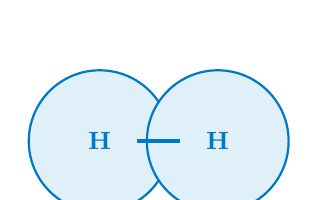
\begin{tikzpicture}[scale=0.6]
        % Simple hydrogen molecule logo
        \draw[thick, h2color, fill=watercolor!20] (0,0) circle (1.5);
        \draw[thick, h2color, fill=watercolor!20] (2.5,0) circle (1.5);
        \draw[very thick, h2color] (0.8,0) -- (1.7,0);
        \node[font=\small\bfseries, h2color] at (0,0) {H};
        \node[font=\small\bfseries, h2color] at (2.5,0) {H};
    \end{tikzpicture}

    \vspace{1cm}

    {\Huge\bfseries Hydrodomus}\\[0.5cm]
    {\Large\itshape Home Hydrogen Generation System\\for Automotive Applications}\\[2cm]

    {\Large\bfseries Technical Specification\\and Business Case}\\[1.5cm]

    \rule{0.8\textwidth}{0.4pt}\\[1.5cm]

    {\large Investor Prospectus}\\[0.3cm]
    {\large Version 2.0}\\[2cm]

    \begin{tabular}{rl}
        \textbf{Author:} & Yannick Durindel \\[0.3cm]
        \textbf{Company:} & Hydrodomus \\[0.3cm]
        \textbf{Date:} & \today \\
    \end{tabular}

    \vfill

    {\small\itshape ``Hydro'' (water) + ``Domus'' (home) = Hydrogen at Home}

\end{titlepage}


\clearpage
\chapter*{Abstract}
\thispagestyle{empty}
The transition to hydrogen-powered transportation faces a critical infrastructure challenge: while hydrogen \gls{fcev} technology has matured to commercial viability, the refueling network remains severely limited compared to conventional fueling stations. This document presents the technical specification for \textbf{Hydrodomus}, a home-based hydrogen generation and storage system designed to address this infrastructure gap by enabling \gls{fcev} owners to produce and store hydrogen fuel at their residence.

The proposed system utilizes \gls{pem} water electrolysis to generate high-purity hydrogen from water and electricity. The produced hydrogen is compressed to the automotive standard pressure of \SI{700}{bar} and stored in a certified composite vessel, from which the user can refuel their vehicle using a standardized SAE J2601-compliant dispensing system.

This document provides comprehensive coverage of the underlying theoretical principles, including electrochemistry, thermodynamics of gas compression, and hydrogen storage physics. The system architecture is presented in detail, with component specifications derived from both commercial availability and technical requirements. Safety considerations and the regulatory certification pathway are thoroughly analyzed to ensure compliance with international standards including ISO 19880, EC 79/2009, and SAE J2601.

The technical analysis demonstrates that home hydrogen generation is feasible with current technology, with system efficiency in the range of 60--70\% from electricity to stored hydrogen. The primary challenges identified include the high capital cost of \SI{700}{bar} compression equipment and storage vessels, as well as the certification requirements for residential hydrogen systems. The document concludes with recommendations for prototype development and a roadmap toward commercial deployment.

\textbf{Keywords:} Hydrogen production, PEM electrolysis, home refueling, FCEV, 700 bar storage, SAE J2601


% Table of Contents
\cleardoublepage
\pagenumbering{roman}
\tableofcontents
\clearpage

% List of Tables
\phantomsection
\listoftables
\addcontentsline{toc}{chapter}{\listtablename}

% List of Figures
\phantomsection
\listoffigures
\addcontentsline{toc}{chapter}{\listfigurename}

\printglossary[title={List of Abbreviations},type=\acronymtype, style=mystyle]
\printglossary[type=symbolslist,style=symbunitlong]

\chapter{Introduction}
\pagenumbering{arabic}
This chapter introduces the context and motivation for home-based hydrogen generation systems. The current state of hydrogen mobility infrastructure is examined, and the fundamental concept of the Hydrodomus system is presented along with the objectives of this technical specification.

\section{The Hydrogen Mobility Challenge}

\subsection{Current State of Hydrogen Vehicles}

Hydrogen \glspl{fcev} represent one of the most promising pathways toward zero-emission transportation. Unlike \glspl{bev}, which store energy in batteries, \glspl{fcev} generate electricity on-board through an electrochemical reaction between hydrogen and oxygen, producing only water as a byproduct. This approach offers several advantages:

\begin{itemize}
    \item \textbf{Rapid refueling}: A full tank can be achieved in 3--5 minutes, comparable to conventional vehicles
    \item \textbf{Long range}: Modern \glspl{fcev} achieve 500--700 km per tank
    \item \textbf{No degradation}: Unlike batteries, fuel cells do not suffer from cycle-dependent capacity loss
    \item \textbf{Weight advantage}: For larger vehicles and long-range applications, hydrogen storage is lighter than equivalent battery capacity
\end{itemize}

Several major automotive manufacturers have invested significantly in \gls{fcev} technology. The Toyota Mirai, now in its second generation, demonstrates the commercial maturity of the technology with a range exceeding \SI{650}{km}. BMW has developed the iX5 Hydrogen, Hyundai offers the Nexo SUV, and various commercial vehicle manufacturers are developing hydrogen-powered trucks and buses.

\paragraph{The Fundamental Problem}

Despite technological maturity, \gls{fcev} adoption faces a critical barrier: the lack of refueling infrastructure. As of 2024, there are approximately 1,000 hydrogen refueling stations worldwide, compared to over 150,000 gasoline stations in the United States alone. This creates the well-known ``chicken-and-egg'' problem:

\begin{itemize}
    \item Consumers hesitate to purchase \glspl{fcev} due to limited refueling options
    \item Infrastructure investors hesitate to build stations due to low vehicle population
    \item Vehicle manufacturers cannot achieve economies of scale without consumer demand
\end{itemize}

This situation contrasts sharply with \glspl{bev}, where home charging provides a baseline capability that mitigates range anxiety. An \gls{bev} owner can always charge at home overnight, even if public charging infrastructure is limited. \gls{fcev} owners have no equivalent option---until now.

\subsection{The Home Refueling Concept}

The Hydrodomus system proposes to break the infrastructure deadlock by bringing hydrogen production directly to the consumer's residence. Just as an \gls{bev} owner plugs in their vehicle overnight, a Hydrodomus owner would generate hydrogen at home using water and electricity.

\begin{figure}[htbp]
    \centering
    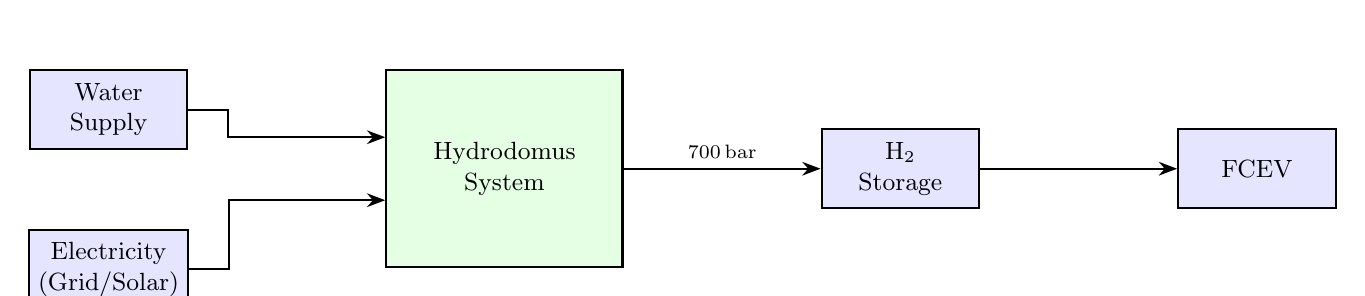
\begin{tikzpicture}[
        node distance=2.5cm,
        block/.style={rectangle, draw, thick, minimum width=2cm, minimum height=1cm, align=center, fill=blue!10, font=\small},
        arrow/.style={-{Stealth}, thick}
    ]
        % Inputs
        \node[block] (water) {Water\\Supply};
        \node[block, below=1cm of water] (elec) {Electricity\\(Grid/Solar)};

        % System
        \node[block, right=of water, yshift=-0.75cm, minimum width=3cm, minimum height=2.5cm, fill=green!10] (system) {Hydrodomus\\System};

        % Output
        \node[block, right=of system] (storage) {H\textsubscript{2}\\Storage};
        \node[block, right=of storage] (vehicle) {FCEV};

        % Arrows
        \draw[arrow] (water.east) -- ++(0.5,0) |- ([yshift=0.4cm]system.west);
        \draw[arrow] (elec.east) -- ++(0.5,0) |- ([yshift=-0.4cm]system.west);
        \draw[arrow] (system) -- node[above, font=\scriptsize] {\SI{700}{bar}} (storage);
        \draw[arrow] (storage) -- (vehicle);

    \end{tikzpicture}
    \caption{Conceptual overview of the Hydrodomus home hydrogen generation system. Water and electricity are converted to compressed hydrogen for vehicle refueling.}
    \label{fig:concept_overview}
\end{figure}

This approach transforms the infrastructure problem from a societal challenge into an individual solution. Each \gls{fcev} owner becomes independent of the public refueling network, at least for routine daily driving. The benefits include:

\begin{itemize}
    \item \textbf{Energy independence}: Users are not dependent on the location or availability of public stations
    \item \textbf{Cost predictability}: Fuel costs depend on electricity prices rather than volatile hydrogen markets
    \item \textbf{Convenience}: Refueling occurs at home, similar to \gls{bev} charging
    \item \textbf{Grid integration}: The system can operate during off-peak hours or use surplus renewable energy
\end{itemize}

\section{Market Context}

\subsection{Existing Solutions}

The concept of home hydrogen generation is not entirely new, though no commercial system currently meets the requirements for automotive refueling at \SI{700}{bar}. Existing approaches include:

\textbf{Industrial electrolyzers}: Large-scale \gls{pem} and alkaline electrolyzers are commercially available from manufacturers such as Nel, ITM Power, and Siemens. These systems are designed for industrial applications and typically produce hydrogen at low pressure (\SI{30}{bar} or less), requiring additional compression for automotive use.

\textbf{Home hydrogen generators}: Several companies have marketed small-scale hydrogen generators for laboratory or backup power applications. These typically operate at atmospheric pressure and produce insufficient quantities for vehicle refueling.

\textbf{Toyota's home hydrogen concept}: Toyota has announced development of a home hydrogen system in Japan, though details remain limited and the system appears targeted at the Japanese market with its specific regulatory environment.

\subsection{Technology Readiness}

The individual components required for a home hydrogen system are all commercially available:

\begin{itemize}
    \item \gls{pem} electrolyzers at the 1--5 kW scale
    \item High-pressure hydrogen compressors capable of \SI{700}{bar}
    \item Type IV composite hydrogen storage vessels
    \item SAE J2601-compliant dispensing nozzles
\end{itemize}

The challenge lies not in developing new technology but in integrating these components into a safe, certified, and cost-effective residential system.

\section{Project Objectives}

\subsection{Technical Objectives}

The Hydrodomus project aims to develop a complete home hydrogen generation system with the following technical specifications:

\begin{enumerate}
    \item \textbf{Hydrogen production}: Minimum \SI{0.5}{kg/day} production capacity using \gls{pem} electrolysis
    \item \textbf{Storage pressure}: \SI{700}{bar} (70 MPa) to match automotive standards
    \item \textbf{Storage capacity}: Minimum \SI{10}{L} at \SI{700}{bar}, equivalent to approximately \SI{0.4}{kg} H\textsubscript{2}
    \item \textbf{Dispensing}: SAE J2601-compliant refueling interface
    \item \textbf{Efficiency}: System efficiency $>$60\% (electricity to stored hydrogen)
    \item \textbf{Safety}: Full compliance with applicable residential and hydrogen safety standards
\end{enumerate}

\subsection{Commercial Objectives}

Beyond technical feasibility, the project must achieve commercial viability:

\begin{itemize}
    \item Target system cost allowing payback within 5--7 years compared to station refueling
    \item Minimal maintenance requirements suitable for residential operation
    \item User-friendly interface requiring no specialized knowledge
    \item Certification pathway enabling legal installation in residential settings
\end{itemize}

\section{Document Structure}

This technical specification is organized as follows:

\textbf{Chapter 2: Theoretical Background} presents the scientific foundations required to understand the system, including electrochemistry of water electrolysis, thermodynamics of hydrogen compression, and gas storage physics.

\textbf{Chapter 3: System Architecture} describes the complete system design, including process flow, subsystem interactions, and control strategy.

\textbf{Chapter 4: Component Specifications} provides detailed requirements for each major component, with reference to commercially available solutions.

\textbf{Chapter 5: Safety and Certifications} analyzes the applicable safety standards and outlines the certification pathway for residential deployment.

\textbf{Chapter 6: Conclusions and Future Work} summarizes the technical findings and identifies next steps for prototype development.


\chapter{Theoretical Background}
This chapter presents the theoretical foundations necessary for understanding the design and operation of the Hydrodomus system. Starting from fundamental electrochemistry, we develop the principles governing water electrolysis, then proceed to the thermodynamics of gas compression and storage. These principles directly inform the engineering decisions presented in subsequent chapters.

\section{Electrochemistry of Water Electrolysis}

\subsection{Fundamental Principles}

Water electrolysis is the process of using electrical energy to decompose water into its constituent elements, hydrogen and oxygen. This electrochemical reaction is the reverse of the hydrogen-oxygen fuel cell reaction and represents a well-understood industrial process with over 200 years of history.

The overall reaction for water splitting is:
\begin{equation}
    \ch{2 H2O_{(l)} -> 2 H2_{(g)} + O2_{(g)}}
    \label{eq:overall_electrolysis}
\end{equation}

This deceptively simple equation conceals significant thermodynamic and kinetic complexity. The reaction is highly endothermic---it requires energy input---and does not occur spontaneously at ambient conditions. The energy required comes from the electrical power supplied to the electrochemical cell.

\paragraph{Why Water Splitting Requires Energy}

The thermodynamic requirement for water splitting can be understood from the perspective of chemical bond energies. In water, each oxygen atom forms two strong covalent bonds with hydrogen atoms. Breaking these O--H bonds requires energy input. While new H--H and O=O bonds form in the products, the total bond energy of the products is less than that required to break the reactant bonds. This energy difference must be supplied externally.

From a thermodynamic standpoint, the Gibbs free energy change for the reaction at standard conditions is:
\begin{equation}
    \Delta G^0 = +\SI{237.1}{kJ/mol}
    \label{eq:gibbs_standard}
\end{equation}

The positive value indicates a non-spontaneous process---energy must be added to drive the reaction forward.

\subsection{Electrode Reactions}

The overall water splitting reaction occurs through two half-reactions at the electrodes of the electrolysis cell. The specific reactions depend on whether the system operates under acidic or alkaline conditions.

\subsubsection{Acidic Conditions (PEM Electrolysis)}

In \gls{pem} electrolysis, the membrane conducts protons (H\textsuperscript{+}) and the electrode reactions are:

\textbf{Anode (Oxygen Evolution Reaction---OER):}
\begin{equation}
    \ch{2 H2O -> O2 + 4 H^+ + 4 e^-} \qquad E^0 = +\SI{1.229}{V}
    \label{eq:oer_acidic}
\end{equation}

\textbf{Cathode (Hydrogen Evolution Reaction---HER):}
\begin{equation}
    \ch{4 H^+ + 4 e^- -> 2 H2} \qquad E^0 = \SI{0.000}{V}
    \label{eq:her_acidic}
\end{equation}

At the anode, water molecules are oxidized, releasing oxygen gas, protons, and electrons. The protons migrate through the membrane to the cathode, while electrons flow through the external circuit. At the cathode, protons combine with electrons to form hydrogen gas.

\subsubsection{Alkaline Conditions}

In alkaline electrolysis, hydroxide ions (OH\textsuperscript{-}) are the mobile ionic species:

\textbf{Cathode:}
\begin{equation}
    \ch{4 H2O + 4 e^- -> 2 H2 + 4 OH^-}
    \label{eq:her_alkaline}
\end{equation}

\textbf{Anode:}
\begin{equation}
    \ch{4 OH^- -> O2 + 2 H2O + 4 e^-}
    \label{eq:oer_alkaline}
\end{equation}

\paragraph{Physical Interpretation}

The electrode reactions reveal why gas separation is inherent to the electrolysis process: hydrogen is produced exclusively at the cathode, while oxygen is produced exclusively at the anode. If the electrodes are physically separated (by a membrane or diaphragm), the gases remain separated and no additional purification is required. This is a fundamental advantage of electrolysis over thermal water splitting methods.

\subsection{Thermodynamics of Electrolysis}

\subsubsection{Minimum Voltage Requirement}

The minimum voltage required to drive electrolysis is determined by the thermodynamics of the reaction. The reversible cell voltage $E_{rev}$ is related to the Gibbs free energy change by:
\begin{equation}
    E_{rev} = \frac{\Delta G}{nF}
    \label{eq:reversible_voltage}
\end{equation}

where $n$ is the number of electrons transferred (4 for the overall reaction) and $F$ is the Faraday constant (\SI{96485}{C/mol}).

At standard conditions:
\begin{equation}
    E_{rev}^0 = \frac{\SI{237100}{J/mol}}{4 \times \SI{96485}{C/mol}} = \SI{1.229}{V}
    \label{eq:standard_voltage}
\end{equation}

This is the theoretical minimum voltage for water electrolysis at \SI{25}{\celsius} and \SI{1}{bar}.

\subsubsection{Thermoneutral Voltage}

In practice, the enthalpy change $\Delta H$ is more relevant than the Gibbs free energy because it accounts for the total energy required, including the entropy term. The thermoneutral voltage is:
\begin{equation}
    E_{tn} = \frac{\Delta H}{nF} = \frac{\SI{285800}{J/mol}}{4 \times \SI{96485}{C/mol}} = \SI{1.481}{V}
    \label{eq:thermoneutral_voltage}
\end{equation}

At voltages below $E_{tn}$, the cell would absorb heat from the surroundings; above $E_{tn}$, the cell generates heat. Practical electrolyzers operate above the thermoneutral voltage due to various losses, meaning they always generate heat that must be managed.

\begin{figure}[htbp]
    \centering
    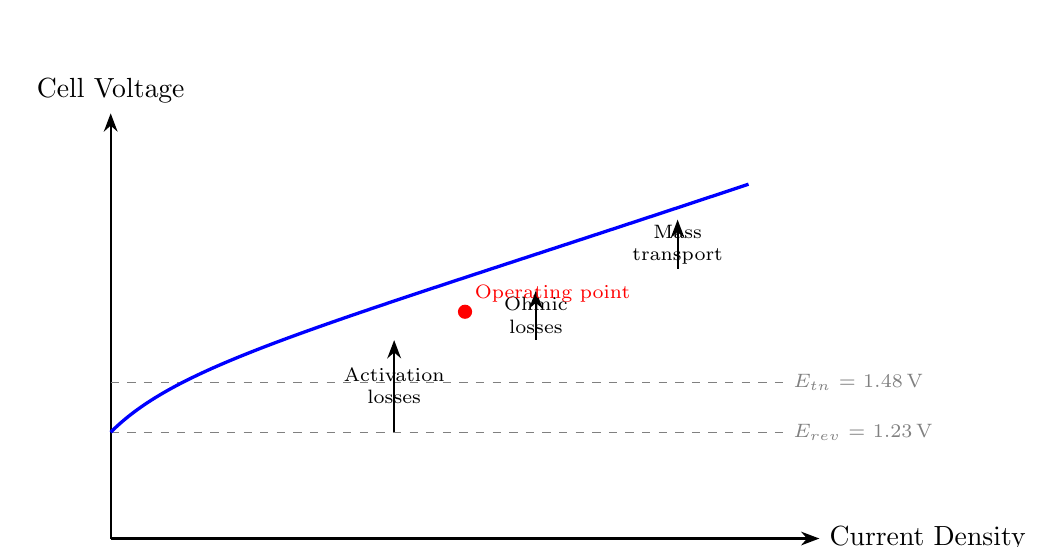
\begin{tikzpicture}[scale=0.9]
        % Axes
        \draw[thick, -{Stealth}] (0,0) -- (10,0) node[right] {Current Density};
        \draw[thick, -{Stealth}] (0,0) -- (0,6) node[above] {Cell Voltage};

        % Voltage levels
        \draw[dashed, gray] (0,1.5) -- (9.5,1.5) node[right, font=\scriptsize] {$E_{rev}$ = \SI{1.23}{V}};
        \draw[dashed, gray] (0,2.2) -- (9.5,2.2) node[right, font=\scriptsize] {$E_{tn}$ = \SI{1.48}{V}};

        % Polarization curve
        \draw[very thick, blue] (0,1.5) .. controls (1,2.5) and (3,3) .. (9,5);

        % Regions
        \draw[{Stealth}-, thick] (4,2.8) -- (4,1.5);
        \node[font=\scriptsize, align=center] at (4,2.15) {Activation\\losses};

        \draw[{Stealth}-, thick] (6,3.5) -- (6,2.8);
        \node[font=\scriptsize, align=center] at (6,3.15) {Ohmic\\losses};

        \draw[{Stealth}-, thick] (8,4.5) -- (8,3.8);
        \node[font=\scriptsize, align=center] at (8,4.15) {Mass\\transport};

        % Operating point
        \fill[red] (5,3.2) circle (0.1);
        \node[above right, red, font=\scriptsize] at (5,3.2) {Operating point};

    \end{tikzpicture}
    \caption{Polarization curve for a water electrolysis cell showing the relationship between cell voltage and current density. The gap between the reversible voltage $E_{rev}$ and the operating voltage represents efficiency losses from activation overpotentials, ohmic resistance, and mass transport limitations.}
    \label{fig:polarization_curve}
\end{figure}

\subsubsection{Overpotentials and Efficiency Losses}

Real electrolysis cells operate at voltages significantly higher than the reversible voltage due to various loss mechanisms:

\textbf{Activation overpotential} ($\eta_{act}$): Energy required to overcome the activation barrier for the electrode reactions. The oxygen evolution reaction has particularly high activation overpotential due to its complex four-electron mechanism.

\textbf{Ohmic overpotential} ($\eta_{\Omega}$): Resistive losses in the membrane/electrolyte, electrodes, and current collectors. This term increases linearly with current density according to Ohm's law:
\begin{equation}
    \eta_{\Omega} = i \cdot R_{cell}
    \label{eq:ohmic_loss}
\end{equation}

\textbf{Mass transport overpotential} ($\eta_{mt}$): At high current densities, the supply of reactants or removal of products can become rate-limiting, causing additional voltage losses.

The total cell voltage is:
\begin{equation}
    E_{cell} = E_{rev} + \eta_{act,a} + \eta_{act,c} + \eta_{\Omega} + \eta_{mt}
    \label{eq:total_voltage}
\end{equation}

\subsubsection{Energy Efficiency}

The voltage efficiency of an electrolyzer is defined as:
\begin{equation}
    \eta_V = \frac{E_{tn}}{E_{cell}}
    \label{eq:voltage_efficiency}
\end{equation}

Using the thermoneutral voltage accounts for the total energy content of the hydrogen produced. Modern \gls{pem} electrolyzers achieve voltage efficiencies of 70--80\% at typical operating conditions.

The specific energy consumption is often expressed as:
\begin{equation}
    E_s = \frac{E_{cell} \cdot n \cdot F}{M_{H_2}} = \frac{E_{cell} \times 2 \times 96485}{2.016 \times 3600} \approx 26.6 \times E_{cell} \quad [\si{kWh/kg}]
    \label{eq:specific_energy}
\end{equation}

For a cell operating at \SI{1.8}{V}, the specific energy consumption is approximately \SI{48}{kWh/kg} of hydrogen.

\subsection{Faraday's Laws of Electrolysis}

Faraday's laws provide the quantitative relationship between electrical charge and the amount of substance produced:

\textbf{First Law}: The mass of substance produced is proportional to the charge passed:
\begin{equation}
    m = \frac{Q \cdot M}{n \cdot F} = \frac{I \cdot t \cdot M}{n \cdot F}
    \label{eq:faraday_first}
\end{equation}

For hydrogen production ($M = \SI{2.016}{g/mol}$, $n = 2$):
\begin{equation}
    m_{H_2} = \frac{I \cdot t \cdot 2.016}{2 \times 96485} = 1.044 \times 10^{-5} \cdot I \cdot t \quad [\si{g}]
    \label{eq:hydrogen_production_rate}
\end{equation}

\paragraph{Practical Implications}

Faraday's law has important practical implications for system design:

\begin{itemize}
    \item A \SI{1}{kW} electrolyzer operating at \SI{1.8}{V} draws approximately \SI{556}{A}
    \item This produces hydrogen at a rate of \SI{20.9}{g/h} or approximately \SI{0.5}{kg/day}
    \item The oxygen production rate is exactly half the molar rate of hydrogen (from stoichiometry)
\end{itemize}

\section{PEM Electrolysis Technology}

\subsection{Operating Principle}

\Gls{pem} electrolysis uses a solid polymer electrolyte---typically a perfluorosulfonic acid membrane such as Nafion---to conduct protons between the electrodes while providing gas separation. The technology was developed from \gls{pem} fuel cell research and offers several advantages for the Hydrodomus application.

\begin{figure}[htbp]
    \centering
    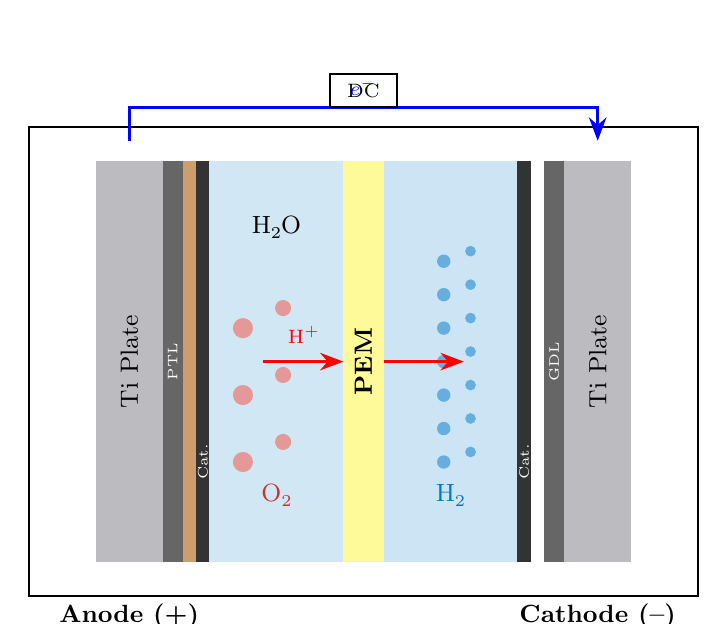
\begin{tikzpicture}[scale=0.85]
        % Frame
        \draw[thick] (0,0) rectangle (10,7);

        % Membrane
        \fill[yellow!40] (4.7,0.5) rectangle (5.3,6.5);
        \node[rotate=90, font=\small\bfseries] at (5,3.5) {PEM};

        % Anode side
        \fill[steelcolor!50] (1,0.5) rectangle (2,6.5);
        \node[rotate=90, font=\small] at (1.5,3.5) {Ti Plate};

        \fill[black!60] (2,0.5) rectangle (2.3,6.5);
        \node[rotate=90, font=\tiny, white] at (2.15,3.5) {PTL};

        \fill[coppercolor!70] (2.3,0.5) rectangle (2.5,6.5);

        \fill[black!80] (2.5,0.5) rectangle (2.7,6.5);
        \node[rotate=90, font=\tiny, white] at (2.6,2) {Cat.};

        % Water/O2 channel
        \fill[watercolor!30] (2.7,0.5) rectangle (4.7,6.5);
        \node[font=\small] at (3.7,5.5) {\ch{H2O}};

        % O2 bubbles
        \foreach \y in {2,3,4} {
            \fill[o2color!50] (3.2,\y) circle (0.15);
            \fill[o2color!50] (3.8,\y+0.3) circle (0.12);
        }
        \node[o2color, font=\small] at (3.7,1.5) {\ch{O2}};

        % Cathode side
        \fill[steelcolor!50] (8,0.5) rectangle (9,6.5);
        \node[rotate=90, font=\small] at (8.5,3.5) {Ti Plate};

        \fill[black!60] (7.7,0.5) rectangle (8,6.5);
        \node[rotate=90, font=\tiny, white] at (7.85,3.5) {GDL};

        \fill[black!80] (7.3,0.5) rectangle (7.5,6.5);
        \node[rotate=90, font=\tiny, white] at (7.4,2) {Cat.};

        % H2 channel
        \fill[h2color!20] (5.3,0.5) rectangle (7.3,6.5);

        % H2 bubbles
        \foreach \y in {2,2.5,3,3.5,4,4.5,5} {
            \fill[h2color!60] (6.2,\y) circle (0.1);
            \fill[h2color!60] (6.6,\y+0.15) circle (0.08);
        }
        \node[h2color, font=\small] at (6.3,1.5) {\ch{H2}};

        % Proton transport
        \draw[-{Stealth}, very thick, red] (3.5,3.5) -- (4.7,3.5);
        \draw[-{Stealth}, very thick, red] (5.3,3.5) -- (6.5,3.5);
        \node[red, font=\scriptsize] at (4.1,3.9) {\ch{H+}};

        % Electron flow
        \draw[-{Stealth}, very thick, blue] (1.5,6.8) -- (1.5,7.3) -- (8.5,7.3) -- (8.5,6.8);
        \node[blue, font=\scriptsize] at (5,7.6) {$e^-$};

        % Labels
        \node[font=\small\bfseries] at (1.5,-0.3) {Anode (+)};
        \node[font=\small\bfseries] at (8.5,-0.3) {Cathode (--)};

        % Power supply
        \draw[thick] (4.5,7.3) rectangle (5.5,7.8);
        \node[font=\scriptsize] at (5,7.55) {DC};

    \end{tikzpicture}
    \caption{Cross-sectional schematic of a \gls{pem} electrolysis cell. Water is fed to the anode where it is oxidized to oxygen and protons. Protons migrate through the membrane to the cathode where they combine with electrons to form hydrogen. The membrane provides inherent gas separation.}
    \label{fig:pem_cell}
\end{figure}

\subsection{Membrane Electrode Assembly}

The \gls{mea} is the core component of a \gls{pem} electrolyzer, consisting of:

\textbf{Proton exchange membrane}: Typically Nafion (perfluorosulfonic acid), 50--200 \si{\micro m} thick. The membrane conducts protons with conductivity of 0.1--0.2 S/cm when hydrated, while being impermeable to gases and electrons.

\textbf{Catalyst layers}: Platinum-based catalysts for the cathode (HER) and iridium oxide for the anode (OER). Catalyst loadings are typically 0.5--2 mg/cm\textsuperscript{2}. The high cost of iridium is a significant contributor to \gls{pem} electrolyzer cost.

\textbf{Porous transport layers}: Gas diffusion layers (GDL) on the cathode side and porous transport layers (PTL) on the anode side facilitate reactant distribution and product removal.

\subsection{Advantages for Home Application}

\Gls{pem} technology offers several advantages that make it well-suited for the Hydrodomus application:

\begin{enumerate}
    \item \textbf{Compact design}: High current densities (1--3 A/cm\textsuperscript{2}) enable small footprint
    \item \textbf{Solid electrolyte}: No liquid caustic chemicals requiring special handling
    \item \textbf{Dynamic response}: Can follow variable power input (suitable for solar integration)
    \item \textbf{High purity output}: Produces >99.99\% pure hydrogen directly
    \item \textbf{Pressurized operation}: Some systems operate at elevated pressure, reducing compression requirements
    \item \textbf{Low maintenance}: No electrolyte management required
\end{enumerate}

\subsection{Performance Characteristics}

Typical performance parameters for commercial \gls{pem} electrolyzers:

\begin{table}[htbp]
    \centering
    \caption{Typical performance parameters for \gls{pem} electrolyzers}
    \label{tab:pem_performance}
    \begin{tabular}{@{}lc@{}}
        \toprule
        \textbf{Parameter} & \textbf{Typical Value} \\
        \midrule
        Cell voltage & 1.7--2.0 V \\
        Current density & 1--3 A/cm\textsuperscript{2} \\
        Operating temperature & 50--80 \si{\celsius} \\
        Operating pressure & 1--30 bar \\
        Specific energy consumption & 50--55 kWh/kg H\textsubscript{2} \\
        System efficiency (LHV) & 60--70\% \\
        Hydrogen purity & >99.99\% \\
        Lifetime & >60,000 hours \\
        \bottomrule
    \end{tabular}
\end{table}

\section{Thermodynamics of Gas Compression}

\subsection{Compression Work}

Compressing hydrogen from electrolyzer output pressure to storage pressure requires mechanical work. The minimum work for isothermal compression of an ideal gas is:
\begin{equation}
    W_{iso} = nRT \ln\left(\frac{p_2}{p_1}\right)
    \label{eq:isothermal_work}
\end{equation}

For compressing \SI{1}{kg} of hydrogen from \SI{1}{bar} to \SI{700}{bar} at \SI{298}{K}:
\begin{equation}
    W_{iso} = \frac{1000}{2.016} \times 8.314 \times 298 \times \ln(700) = \SI{8.07}{MJ} = \SI{2.24}{kWh}
    \label{eq:compression_work_calc}
\end{equation}

\subsection{Real Gas Effects}

At high pressures, hydrogen deviates significantly from ideal gas behavior. The compressibility factor $Z$ accounts for these deviations:
\begin{equation}
    pV = ZnRT
    \label{eq:real_gas}
\end{equation}

For hydrogen at \SI{700}{bar} and \SI{25}{\celsius}, $Z \approx 1.5$, meaning the gas occupies 50\% more volume than predicted by the ideal gas law. This has important implications:

\begin{itemize}
    \item More compression work is required than the ideal gas calculation suggests
    \item Storage capacity is less than ideal gas predictions
    \item Density at \SI{700}{bar} is approximately \SI{40}{kg/m^3} rather than the ideal \SI{57}{kg/m^3}
\end{itemize}

\begin{figure}[htbp]
    \centering
    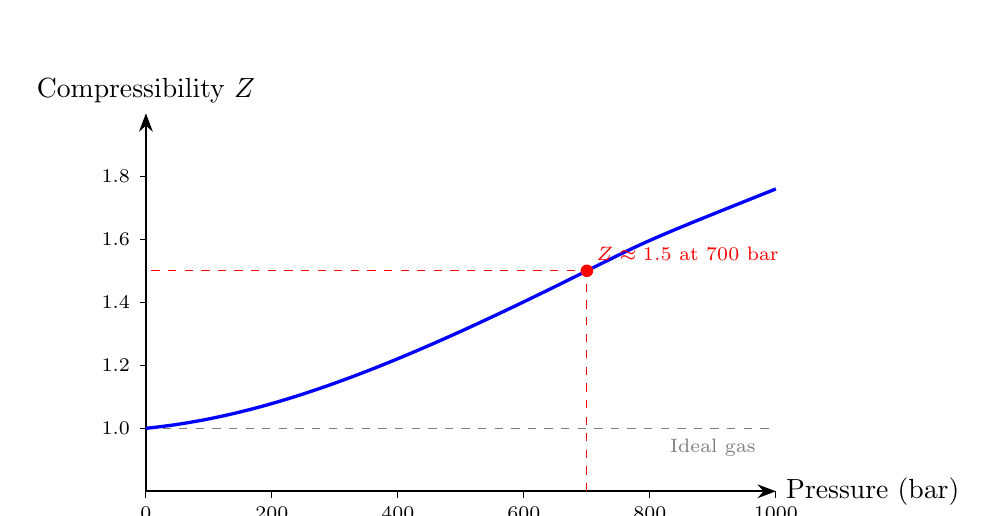
\begin{tikzpicture}[scale=0.8]
        % Axes
        \draw[thick, -{Stealth}] (0,0) -- (10,0) node[right] {Pressure (bar)};
        \draw[thick, -{Stealth}] (0,0) -- (0,6) node[above] {Compressibility $Z$};

        % Tick marks
        \foreach \x/\label in {0/0, 2/200, 4/400, 6/600, 8/800, 10/1000} {
            \draw (\x,0) -- (\x,-0.1) node[below, font=\scriptsize] {\label};
        }
        \foreach \y/\label in {1/1.0, 2/1.2, 3/1.4, 4/1.6, 5/1.8} {
            \draw (0,\y) -- (-0.1,\y) node[left, font=\scriptsize] {\label};
        }

        % Z = 1 reference
        \draw[dashed, gray] (0,1) -- (10,1);
        \node[gray, font=\scriptsize] at (9,0.7) {Ideal gas};

        % Compressibility curve (approximate)
        \draw[very thick, blue] (0,1) .. controls (2,1.2) and (4,2) .. (7,3.5) .. controls (8,4) .. (10,4.8);

        % 700 bar point
        \fill[red] (7,3.5) circle (0.1);
        \draw[dashed, red] (7,0) -- (7,3.5) -- (0,3.5);
        \node[red, font=\scriptsize, above right] at (7,3.5) {$Z \approx 1.5$ at 700 bar};

    \end{tikzpicture}
    \caption{Compressibility factor $Z$ for hydrogen as a function of pressure at \SI{25}{\celsius}. At \SI{700}{bar}, hydrogen deviates significantly from ideal gas behavior with $Z \approx 1.5$.}
    \label{fig:compressibility}
\end{figure}

\subsection{Compression Efficiency}

Real compressors operate closer to adiabatic than isothermal conditions, especially at high compression ratios. For multi-stage adiabatic compression with intercooling:
\begin{equation}
    W_{adi} = \frac{\gamma}{\gamma-1} \cdot nRT_1 \cdot N \left[\left(\frac{p_2}{p_1}\right)^{\frac{\gamma-1}{N\gamma}} - 1\right]
    \label{eq:adiabatic_work}
\end{equation}

where $N$ is the number of compression stages and $\gamma = 1.41$ for hydrogen.

Including mechanical inefficiencies, practical compression energy is typically 3--5 kWh/kg for compression from \SI{30}{bar} to \SI{700}{bar}.

\section{Hydrogen Storage}

\subsection{Storage Methods Overview}

Hydrogen can be stored in several forms:

\begin{itemize}
    \item \textbf{Compressed gas}: Most mature technology, used in vehicles
    \item \textbf{Liquid hydrogen}: Higher density but requires cryogenic temperatures (\SI{20}{K})
    \item \textbf{Metal hydrides}: Solid-state storage with high volumetric density but heavy
    \item \textbf{Chemical carriers}: Ammonia, methanol, or liquid organic hydrogen carriers
\end{itemize}

For the Hydrodomus application, compressed gas storage at \SI{700}{bar} is the appropriate choice as it matches the automotive standard.

\subsection{Compressed Gas Storage}

\subsubsection{Pressure-Volume Relationship}

The amount of hydrogen stored in a vessel depends on pressure, temperature, and vessel volume. Using the real gas equation:
\begin{equation}
    m = \frac{pVM}{ZRT}
    \label{eq:stored_mass}
\end{equation}

For a \SI{10}{L} vessel at \SI{700}{bar} and \SI{25}{\celsius}:
\begin{equation}
    m = \frac{700 \times 10^5 \times 0.01 \times 2.016 \times 10^{-3}}{1.5 \times 8.314 \times 298} = \SI{0.38}{kg}
    \label{eq:stored_mass_calc}
\end{equation}

This represents approximately 7\% of a Toyota Mirai's full tank capacity (\SI{5.6}{kg}).

\subsubsection{Storage Vessel Types}

High-pressure hydrogen vessels are classified into four types:

\begin{table}[htbp]
    \centering
    \caption{Hydrogen storage vessel classification}
    \label{tab:vessel_types}
    \begin{tabular}{@{}clcc@{}}
        \toprule
        \textbf{Type} & \textbf{Construction} & \textbf{Max Pressure} & \textbf{Application} \\
        \midrule
        I & All-metal (steel) & 200--300 bar & Industrial \\
        II & Metal liner + composite hoop wrap & 300--450 bar & Industrial \\
        III & Metal liner + full composite wrap & 350--700 bar & Vehicles, stationary \\
        IV & Polymer liner + full composite wrap & 700 bar & Vehicles \\
        \bottomrule
    \end{tabular}
\end{table}

Type IV vessels, using a high-density polyethylene (HDPE) liner with carbon fiber reinforced polymer (CFRP) overwrap, are standard for \SI{700}{bar} automotive applications. These vessels are designed to fail safely through controlled leakage rather than catastrophic rupture.

\subsection{Safety Considerations}

\subsubsection{Physical Properties of Hydrogen}

Understanding hydrogen's physical properties is essential for safe system design:

\begin{table}[htbp]
    \centering
    \caption{Physical and safety properties of hydrogen compared to other fuels}
    \label{tab:hydrogen_properties}
    \begin{tabular}{@{}lccc@{}}
        \toprule
        \textbf{Property} & \textbf{Hydrogen} & \textbf{Methane} & \textbf{Gasoline} \\
        \midrule
        Density at STP (kg/m\textsuperscript{3}) & 0.0899 & 0.717 & 720--780 \\
        \Gls{lel} (vol\%) & 4.0 & 5.0 & 1.0 \\
        \Gls{uel} (vol\%) & 75 & 15 & 7.6 \\
        Auto-ignition temp. (\si{\celsius}) & 585 & 540 & 230--480 \\
        Min. ignition energy (mJ) & 0.02 & 0.29 & 0.24 \\
        Flame velocity (m/s) & 2.65 & 0.37 & 0.37 \\
        Diffusion coeff. in air (cm\textsuperscript{2}/s) & 0.61 & 0.16 & 0.05 \\
        \bottomrule
    \end{tabular}
\end{table}

\paragraph{Implications for Safety Design}

Several properties have important safety implications:

\begin{itemize}
    \item \textbf{Wide flammability range}: Hydrogen can ignite over a broad range of concentrations, but this also means it disperses to below flammable concentrations more readily than other fuels
    \item \textbf{Low ignition energy}: Eliminates static discharge as a potential ignition source requirement
    \item \textbf{High diffusivity}: Hydrogen disperses rapidly in open environments, reducing accumulation risk
    \item \textbf{Buoyancy}: Being 14 times lighter than air, hydrogen rises rapidly, making outdoor releases relatively safe
    \item \textbf{No toxicity}: Unlike carbon monoxide, hydrogen is non-toxic; the primary hazard is asphyxiation in confined spaces
\end{itemize}

\subsubsection{Deflagration vs. Detonation}

A critical safety distinction exists between deflagration (subsonic flame propagation) and detonation (supersonic). Hydrogen-air mixtures can detonate under specific conditions, but detonation requires:

\begin{itemize}
    \item Concentration near stoichiometric (29\%)
    \item Confinement
    \item Strong ignition source or long flame path
\end{itemize}

In open or well-ventilated environments, hydrogen fires typically deflagrate rather than detonate, producing less destructive overpressure.

\section{Energy Balance}

\subsection{System Efficiency}

The overall efficiency of the Hydrodomus system can be expressed as:
\begin{equation}
    \eta_{system} = \eta_{electrolyzer} \times \eta_{compression} \times \eta_{storage}
    \label{eq:system_efficiency}
\end{equation}

With typical values:
\begin{itemize}
    \item $\eta_{electrolyzer} = 70\%$ (based on LHV)
    \item $\eta_{compression} = 90\%$ (mechanical efficiency)
    \item $\eta_{storage} = 98\%$ (accounting for minor leakage)
\end{itemize}

The overall system efficiency is approximately 62\%.

\subsection{Energy Requirements}

For producing \SI{1}{kg} of hydrogen at \SI{700}{bar}:

\begin{table}[htbp]
    \centering
    \caption{Energy breakdown for producing \SI{1}{kg} of stored hydrogen}
    \label{tab:energy_breakdown}
    \begin{tabular}{@{}lc@{}}
        \toprule
        \textbf{Process} & \textbf{Energy (kWh/kg)} \\
        \midrule
        Electrolysis (at 70\% efficiency) & 47.6 \\
        Compression (30 bar $\rightarrow$ 700 bar) & 3--5 \\
        Balance of plant & 1--2 \\
        \midrule
        \textbf{Total} & \textbf{52--55} \\
        \bottomrule
    \end{tabular}
\end{table}

The \gls{lhv} of hydrogen is \SI{33.3}{kWh/kg}, so the electricity-to-hydrogen efficiency is:
\begin{equation}
    \eta = \frac{33.3}{54} \approx 62\%
    \label{eq:overall_efficiency}
\end{equation}


\chapter{System Architecture}
This chapter presents the complete system architecture for the Hydrodomus home hydrogen generation system. The design philosophy emphasizes safety, modularity, and ease of installation while meeting the technical requirements established in Chapter 1.

\section{System Overview}

\subsection{Functional Description}

The Hydrodomus system performs four primary functions:

\begin{enumerate}
    \item \textbf{Hydrogen generation}: Electrolyze water to produce hydrogen gas
    \item \textbf{Gas separation and purification}: Separate hydrogen from oxygen and water vapor
    \item \textbf{Compression}: Increase hydrogen pressure to \SI{700}{bar}
    \item \textbf{Storage and dispensing}: Store compressed hydrogen and transfer to vehicle
\end{enumerate}

These functions are implemented through five interconnected subsystems, as shown in Figure~\ref{fig:system_block}.

\begin{figure}[htbp]
    \centering
    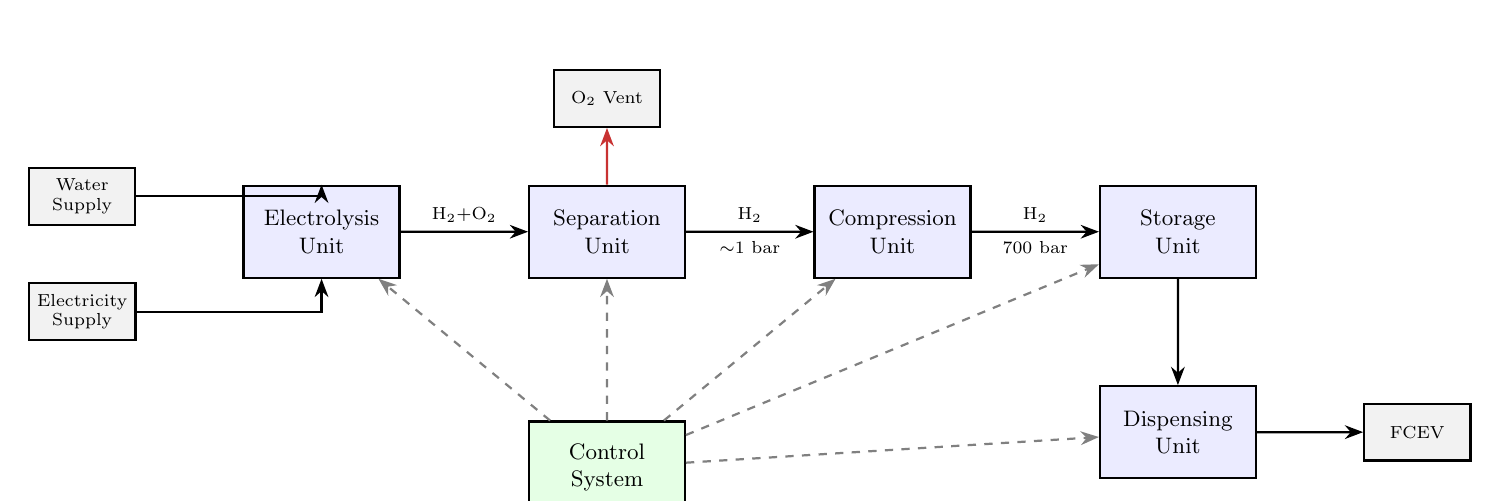
\begin{tikzpicture}[scale=0.9, transform shape,
        node distance=1.8cm,
        block/.style={rectangle, draw, thick, minimum width=2.2cm, minimum height=1.3cm, align=center, fill=blue!8, font=\small},
        smallblock/.style={rectangle, draw, thick, minimum width=1.5cm, minimum height=0.8cm, align=center, fill=gray!10, font=\scriptsize},
        arrow/.style={-{Stealth}, thick},
        dashedarrow/.style={-{Stealth}, thick, dashed}
    ]
        % Input blocks
        \node[smallblock] (water) {Water\\Supply};
        \node[smallblock, below=0.8cm of water] (power) {Electricity\\Supply};

        % Main blocks
        \node[block, right=1.5cm of water, yshift=-0.5cm] (electro) {Electrolysis\\Unit};
        \node[block, right=of electro] (sep) {Separation\\Unit};
        \node[block, right=of sep] (comp) {Compression\\Unit};
        \node[block, right=of comp] (storage) {Storage\\Unit};
        \node[block, below=1.5cm of storage] (disp) {Dispensing\\Unit};

        % Output
        \node[smallblock, right=1.5cm of disp] (vehicle) {FCEV};

        % Control system
        \node[block, below=2cm of sep, fill=green!10] (control) {Control\\System};

        % Vent
        \node[smallblock, above=0.8cm of sep] (vent) {O$_2$ Vent};

        % Arrows for main flow
        \draw[arrow] (water) -| (electro);
        \draw[arrow] (power) -| (electro);
        \draw[arrow] (electro) -- node[above, font=\scriptsize] {H$_2$+O$_2$} (sep);
        \draw[arrow] (sep) -- node[above, font=\scriptsize] {H$_2$} node[below, font=\scriptsize] {$\sim$1 bar} (comp);
        \draw[arrow] (comp) -- node[above, font=\scriptsize] {H$_2$} node[below, font=\scriptsize] {700 bar} (storage);
        \draw[arrow] (storage) -- (disp);
        \draw[arrow] (disp) -- (vehicle);

        % O2 vent
        \draw[arrow, o2color] (sep) -- (vent);

        % Control connections
        \draw[dashedarrow, gray] (control) -- (electro);
        \draw[dashedarrow, gray] (control) -- (sep);
        \draw[dashedarrow, gray] (control) -- (comp);
        \draw[dashedarrow, gray] (control) -- (storage);
        \draw[dashedarrow, gray] (control) -- (disp);

    \end{tikzpicture}
    \caption{Hydrodomus system block diagram showing the five main subsystems and their interconnections. Solid arrows indicate gas flow; dashed arrows indicate control signals.}
    \label{fig:system_block}
\end{figure}

\subsection{Design Philosophy}

The system design follows several key principles:

\textbf{Safety first}: All design decisions prioritize safety. The system includes multiple layers of protection against hydrogen release and operates fail-safe in all identified failure modes.

\textbf{Modularity}: Each subsystem is designed as a replaceable module, enabling maintenance and future upgrades without complete system replacement.

\textbf{Residential compatibility}: The system is designed for installation in a residential garage or utility space, with consideration for noise, footprint, and electrical requirements.

\textbf{Autonomous operation}: Once started, the system operates automatically with minimal user intervention, similar to a home appliance.

\section{Process Flow}

\subsection{Normal Operation Sequence}

The standard operating sequence proceeds as follows:

\textbf{Phase 1: Startup}
\begin{enumerate}
    \item System performs self-check (sensor verification, leak detection)
    \item Water level verified in reservoir
    \item Electrical supply verified
    \item Control system initializes all subsystems
\end{enumerate}

\textbf{Phase 2: Production}
\begin{enumerate}
    \item Electrolyzer powered up, reaching operating temperature
    \item Water fed to electrolyzer at controlled rate
    \item Hydrogen and oxygen produced at electrodes
    \item Gases separated; oxygen vented safely
    \item Hydrogen flows to low-pressure buffer
\end{enumerate}

\textbf{Phase 3: Compression}
\begin{enumerate}
    \item When buffer pressure reaches setpoint, compressor activates
    \item Multi-stage compression to \SI{700}{bar}
    \item Intercooling between stages
    \item Compressed hydrogen flows to storage vessel
\end{enumerate}

\textbf{Phase 4: Standby}
\begin{enumerate}
    \item When storage reaches target pressure, production pauses
    \item System enters low-power standby mode
    \item Monitoring continues for safety parameters
\end{enumerate}

\textbf{Phase 5: Dispensing}
\begin{enumerate}
    \item User connects nozzle to vehicle
    \item System verifies connection integrity
    \item Controlled pressure release to vehicle tank
    \item Flow terminated when vehicle tank full or user stops
\end{enumerate}

\subsection{Process and Instrumentation}

Figure~\ref{fig:pid} presents the detailed process flow with instrumentation points.

\begin{figure}[htbp]
    \centering
    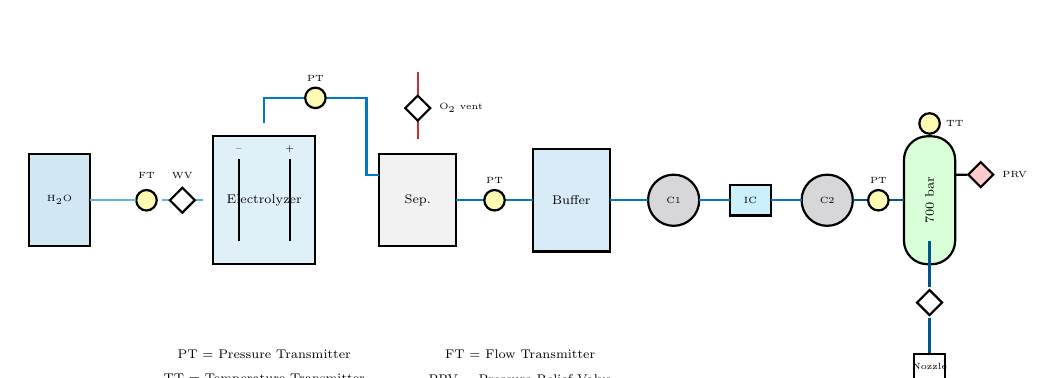
\begin{tikzpicture}[scale=0.65, transform shape,
        tank/.style={rectangle, draw, thick, minimum width=1.2cm, minimum height=1.8cm},
        valve/.style={diamond, draw, thick, minimum size=0.5cm, fill=white},
        pump/.style={circle, draw, thick, minimum size=0.7cm},
        sensor/.style={circle, draw, thick, minimum size=0.4cm, fill=yellow!30},
        arrow/.style={-{Stealth}, thick}
    ]
        % Electrolyzer
        \node[tank, fill=watercolor!20, minimum width=2cm, minimum height=2.5cm] (elec) at (0,0) {};
        \node[font=\scriptsize] at (0,0) {Electrolyzer};

        % Electrodes in electrolyzer
        \draw[thick] (-0.5,-0.8) -- (-0.5,0.8);
        \draw[thick] (0.5,-0.8) -- (0.5,0.8);
        \node[font=\tiny] at (-0.5,1) {--};
        \node[font=\tiny] at (0.5,1) {+};

        % Water inlet
        \draw[thick, watercolor] (-2,0) -- (-1.2,0);
        \node[valve] (wv) at (-1.6,0) {};
        \node[font=\tiny, above] at (-1.6,0.3) {WV};
        \node[sensor] (wf) at (-2.3,0) {};
        \node[font=\tiny, above] at (-2.3,0.3) {FT};

        % Water tank
        \node[tank, fill=watercolor!30] (wtank) at (-4,0) {};
        \node[font=\tiny] at (-4,0) {H$_2$O};
        \draw[thick, watercolor] (-3.4,0) -- (-2.5,0);

        % Separator
        \node[tank, fill=gray!10, minimum width=1.5cm] (sep) at (3,0) {};
        \node[font=\scriptsize] at (3,0) {Sep.};

        % H2 line from electrolyzer
        \draw[thick, h2color] (0,1.5) -- (0,2) -- (2,2) -- (2,0.5) -- (2.25,0.5);
        \node[sensor] (pt1) at (1,2) {};
        \node[font=\tiny, above] at (1,2.2) {PT};

        % O2 vent
        \draw[thick, o2color] (3,1.2) -- (3,2.5);
        \node[valve] (o2v) at (3,1.8) {};
        \node[font=\tiny, right] at (3.3,1.8) {O$_2$ vent};

        % Buffer tank
        \node[tank, fill=h2color!15, minimum width=1.5cm, minimum height=2cm] (buffer) at (6,0) {};
        \node[font=\scriptsize] at (6,0) {Buffer};
        \draw[thick, h2color] (3.75,0) -- (5.25,0);
        \node[sensor] (pt2) at (4.5,0) {};
        \node[font=\tiny, above] at (4.5,0.2) {PT};

        % Compressor (multi-stage)
        \node[pump, fill=steelcolor!30, minimum size=1cm] (comp1) at (8,0) {};
        \node[font=\tiny] at (8,0) {C1};
        \draw[thick, h2color] (6.75,0) -- (7.5,0);

        % Intercooler
        \node[rectangle, draw, thick, minimum width=0.8cm, minimum height=0.6cm, fill=cyan!20] (ic) at (9.5,0) {};
        \node[font=\tiny] at (9.5,0) {IC};
        \draw[thick, h2color] (8.5,0) -- (9.1,0);

        % Second stage
        \node[pump, fill=steelcolor!30, minimum size=1cm] (comp2) at (11,0) {};
        \node[font=\tiny] at (11,0) {C2};
        \draw[thick, h2color] (9.9,0) -- (10.5,0);

        % High pressure storage
        \node[tank, fill=green!15, minimum width=1cm, minimum height=2.5cm, rounded corners=0.3cm] (hptank) at (13,0) {};
        \node[font=\scriptsize, rotate=90] at (13,0) {700 bar};
        \draw[thick, h2color!70!black] (11.5,0) -- (12.5,0);
        \node[sensor] (pt3) at (12,0) {};
        \node[font=\tiny, above] at (12,0.2) {PT};
        \node[sensor] (tt) at (13,1.5) {};
        \node[font=\tiny, right] at (13.2,1.5) {TT};

        % Dispensing
        \node[valve] (dv) at (13,-2) {};
        \draw[thick, h2color!70!black] (13,-0.8) -- (13,-1.7);
        \draw[thick, h2color!70!black] (13,-2.3) -- (13,-3);

        % Nozzle
        \draw[thick] (12.7,-3) -- (13.3,-3) -- (13.3,-3.5) -- (12.7,-3.5) -- cycle;
        \node[font=\tiny] at (13,-3.25) {Nozzle};

        % PRV
        \node[valve, fill=red!20] (prv) at (14,0.5) {};
        \draw[thick] (13.5,0.5) -- (prv);
        \node[font=\tiny, right] at (14.3,0.5) {PRV};

        % Legend
        \node[font=\scriptsize] at (0,-3) {PT = Pressure Transmitter};
        \node[font=\scriptsize] at (0,-3.5) {TT = Temperature Transmitter};
        \node[font=\scriptsize] at (5,-3) {FT = Flow Transmitter};
        \node[font=\scriptsize] at (5,-3.5) {PRV = Pressure Relief Valve};

    \end{tikzpicture}
    \caption{Process and instrumentation diagram (P\&ID) showing major equipment and instrumentation. Blue lines indicate hydrogen flow; equipment labeled with standard ISA symbols.}
    \label{fig:pid}
\end{figure}

\section{Subsystem Descriptions}

\subsection{Electrolysis Unit}

The electrolysis unit generates hydrogen and oxygen from water using \gls{pem} technology.

\textbf{Key specifications:}
\begin{itemize}
    \item Stack power: 1--2 kW nominal
    \item Operating pressure: 1--5 bar (atmospheric to slightly elevated)
    \item Operating temperature: 50--80\si{\celsius}
    \item Water consumption: $\sim$\SI{1}{L/h} at full power
    \item Hydrogen output: $\sim$\SI{20}{g/h} at full power
\end{itemize}

The electrolyzer includes:
\begin{itemize}
    \item \Gls{pem} stack with integrated cooling
    \item Water circulation system with deionization
    \item Power electronics (DC power supply)
    \item Gas-liquid separators for each electrode
\end{itemize}

\subsection{Separation Unit}

The separation unit ensures high-purity hydrogen by removing:
\begin{itemize}
    \item Residual oxygen (if any crossover through membrane)
    \item Water vapor
    \item Trace contaminants
\end{itemize}

For \gls{pem} electrolysis, the membrane provides inherent separation, so this unit primarily performs:
\begin{itemize}
    \item Water knockout (condensation)
    \item Drying (desiccant or refrigerated)
    \item Oxygen venting (with flame arrestor)
\end{itemize}

\subsection{Compression Unit}

The compression unit increases hydrogen pressure from electrolyzer output ($\sim$1--5 bar) to storage pressure (\SI{700}{bar}).

\textbf{Compression approach:}

Multi-stage reciprocating (piston) compression is the only practical technology for achieving \SI{700}{bar} at the required flow rates. A typical configuration uses:

\begin{itemize}
    \item Stage 1: 1--5 bar $\rightarrow$ 30--50 bar
    \item Stage 2: 30--50 bar $\rightarrow$ 200--250 bar
    \item Stage 3: 200--250 bar $\rightarrow$ 700 bar
\end{itemize}

Intercoolers between stages prevent excessive temperature rise during compression. The hydrogen temperature must be controlled to prevent damage to downstream components and storage vessels.

\textbf{Alternative technologies considered:}

\begin{itemize}
    \item \textbf{Ionic compressors}: Use ionic liquid as piston; lower maintenance but limited availability
    \item \textbf{Metal hydride compressors}: Thermal cycling of hydrides; no moving parts but slow
    \item \textbf{Electrochemical compression}: Integrated with electrolyzer; emerging technology
\end{itemize}

\subsection{Storage Unit}

The storage unit holds compressed hydrogen until dispensing. Key requirements:

\begin{itemize}
    \item Vessel type: Type III or Type IV composite
    \item Working pressure: \SI{700}{bar}
    \item Volume: 10--50 L (depending on usage pattern)
    \item Safety features: \gls{tprd}, pressure relief valve, burst disc
\end{itemize}

The storage vessel includes a valve assembly with:
\begin{itemize}
    \item Manual isolation valve
    \item Solenoid-operated fill valve
    \item Check valve (prevent backflow)
    \item \Gls{tprd} for fire protection
    \item Pressure transducer
\end{itemize}

\subsection{Dispensing Unit}

The dispensing unit transfers hydrogen from storage to the vehicle. It must comply with SAE J2601 fueling protocols.

\textbf{SAE J2601 requirements:}
\begin{itemize}
    \item Pre-cooling: Vehicle tanks require cooled hydrogen to prevent overheating during fast fill
    \item Pressure ramp rate: Controlled to prevent thermal stress
    \item Communication: Protocol for determining vehicle tank state
    \item Nozzle standard: ISO 17268 Type B (\SI{700}{bar})
\end{itemize}

For home application, the ``slow fill'' protocol is appropriate:
\begin{itemize}
    \item Fill time: 10--30 minutes (vs. 3--5 minutes at stations)
    \item No pre-cooling required
    \item Simpler pressure management
    \item Lower equipment cost
\end{itemize}

\section{Control System}

\subsection{Control Architecture}

The control system manages all subsystem operations through a hierarchical architecture:

\textbf{Level 1 - Safety systems}: Hardwired safety interlocks that operate independently of software
\begin{itemize}
    \item Emergency stop circuits
    \item Hydrogen detector alarms
    \item Overpressure relief
    \item Fire detection
\end{itemize}

\textbf{Level 2 - Process control}: PLC-based automation
\begin{itemize}
    \item Electrolyzer power management
    \item Compressor sequencing
    \item Pressure and temperature control
    \item Fill protocol execution
\end{itemize}

\textbf{Level 3 - User interface}: Touch screen or app-based interface
\begin{itemize}
    \item System status display
    \item Start/stop commands
    \item Schedule programming
    \item Maintenance alerts
\end{itemize}

\subsection{Operating Modes}

\textbf{Production mode}: System actively generating and compressing hydrogen
\begin{itemize}
    \item Electrolyzer at set power level
    \item Compressor cycling to maintain buffer pressure
    \item Storage pressure increasing
\end{itemize}

\textbf{Standby mode}: Storage full, system idle
\begin{itemize}
    \item Electrolyzer off
    \item Compressor off
    \item Safety monitoring active
    \item Ready for dispensing
\end{itemize}

\textbf{Dispensing mode}: Transferring hydrogen to vehicle
\begin{itemize}
    \item Production may continue simultaneously
    \item Controlled pressure release
    \item Fill protocol management
\end{itemize}

\textbf{Maintenance mode}: System isolated for service
\begin{itemize}
    \item All processes stopped
    \item Valves in safe positions
    \item Technician access enabled
\end{itemize}

\section{Original Concept Sketch}

Figure~\ref{fig:original_sketch} shows the original concept sketch developed during the initial design phase, illustrating the basic system layout and component arrangement.

\begin{figure}[htbp]
    \centering
    \includegraphics[width=0.85\textwidth]{schemalist.jpeg}
    \caption{Original hand-drawn concept sketch showing the proposed system layout. The sketch illustrates the electrolysis tank with electrodes and separator, low-pressure buffer, compressor, high-pressure storage vessel, and connection to vehicle. Component list visible on right side.}
    \label{fig:original_sketch}
\end{figure}

\section{Installation Considerations}

\subsection{Space Requirements}

The complete system is designed to fit within a residential garage or utility space:

\begin{table}[htbp]
    \centering
    \caption{Estimated system dimensions and space requirements}
    \label{tab:space_requirements}
    \begin{tabular}{@{}lcc@{}}
        \toprule
        \textbf{Component} & \textbf{Dimensions (cm)} & \textbf{Floor Space (m$^2$)} \\
        \midrule
        Electrolyzer unit & 60 $\times$ 40 $\times$ 80 & 0.24 \\
        Compressor unit & 80 $\times$ 60 $\times$ 100 & 0.48 \\
        Storage vessel (10 L) & 20 dia $\times$ 80 & 0.04 \\
        Control cabinet & 40 $\times$ 30 $\times$ 60 & 0.12 \\
        \midrule
        \textbf{Total footprint} & & $\sim$\textbf{1.5} \\
        \textbf{Service clearance} & & $\sim$\textbf{1.0} \\
        \bottomrule
    \end{tabular}
\end{table}

\subsection{Utilities}

\textbf{Electrical:}
\begin{itemize}
    \item Supply: 240 V single-phase or 400 V three-phase
    \item Power: 3--5 kW peak, 2 kW average during production
    \item Metering: Separate sub-meter recommended for energy tracking
\end{itemize}

\textbf{Water:}
\begin{itemize}
    \item Connection: Standard household supply
    \item Quality: Tap water acceptable; internal treatment provides deionization
    \item Consumption: $\sim$\SI{10}{L/day} at full production
\end{itemize}

\textbf{Ventilation:}
\begin{itemize}
    \item Requirement: Minimum 0.5 ACH (air changes per hour) when operating
    \item Natural ventilation may be sufficient for well-ventilated garages
    \item Forced ventilation recommended for enclosed spaces
\end{itemize}

\subsection{Environmental Conditions}

\begin{itemize}
    \item Operating temperature: 5--40\si{\celsius}
    \item Storage temperature: --20--50\si{\celsius}
    \item Humidity: 20--80\% RH (non-condensing)
    \item Protection class: IP54 minimum for outdoor-rated components
\end{itemize}


\chapter{Component Specifications}
This chapter provides detailed specifications for the major components of the Hydrodomus system. For each component, design requirements are established based on the system architecture, and commercially available solutions are identified where possible.

\section{Component Overview}

Table~\ref{tab:component_summary} summarizes the major components derived from the original concept sketch and engineering analysis.

\begin{table}[htbp]
    \centering
    \caption{Summary of major system components}
    \label{tab:component_summary}
    \begin{tabular}{@{}clp{6cm}@{}}
        \toprule
        \textbf{No.} & \textbf{Component} & \textbf{Function} \\
        \midrule
        1 & Electrolysis tank (Cuve) & Water container and electrochemical cell \\
        2 & Electrodes & Anode and cathode for water splitting \\
        3 & Separator membrane & Gas separation between H$_2$ and O$_2$ \\
        4 & Electrolyte/Water & Reactant and ionic conductor \\
        5 & Low-pressure tubing & Gas transport at low pressure \\
        6 & Low-pressure reservoir & Buffer storage before compression \\
        7 & High-pressure compressor & Compression to \SI{700}{bar} \\
        8 & Storage vessel & High-pressure hydrogen storage \\
        9 & Dispensing nozzle & Vehicle connection interface \\
        10 & Control system & System automation and safety \\
        \bottomrule
    \end{tabular}
\end{table}

\section{Electrolysis Stack}

\subsection{Requirements}

The electrolyzer must meet the following requirements:

\begin{table}[htbp]
    \centering
    \caption{Electrolyzer requirements}
    \label{tab:electrolyzer_req}
    \begin{tabular}{@{}lcc@{}}
        \toprule
        \textbf{Parameter} & \textbf{Minimum} & \textbf{Target} \\
        \midrule
        Production rate & 0.3 kg/day & 0.5 kg/day \\
        Electrical power & 1.5 kW & 2.0 kW \\
        Efficiency (LHV basis) & 60\% & 70\% \\
        Output pressure & 1 bar & 5--30 bar \\
        Hydrogen purity & 99.9\% & 99.99\% \\
        Lifetime & 40,000 h & 60,000 h \\
        \bottomrule
    \end{tabular}
\end{table}

\subsection{Technology Selection}

\Gls{pem} electrolysis is selected over alkaline electrolysis for the following reasons:

\begin{enumerate}
    \item \textbf{No liquid electrolyte}: Eliminates handling of caustic KOH solution
    \item \textbf{Compact footprint}: Higher current density enables smaller stack
    \item \textbf{Dynamic response}: Suitable for variable renewable input
    \item \textbf{High purity output}: No electrolyte contamination
    \item \textbf{Elevated pressure operation}: Some stacks operate at 30+ bar, reducing compression
\end{enumerate}

\subsection{Commercial Options}

Several manufacturers offer \gls{pem} electrolyzer stacks in the target power range:

\begin{table}[htbp]
    \centering
    \caption{Representative commercial \gls{pem} electrolyzer options}
    \label{tab:electrolyzer_options}
    \begin{tabular}{@{}lcccc@{}}
        \toprule
        \textbf{Manufacturer} & \textbf{Model} & \textbf{Power} & \textbf{Output} & \textbf{Pressure} \\
        \midrule
        Nel & M Series & 1--2 kW & 0.4 Nm$^3$/h & 30 bar \\
        ITM Power & HGAS & 0.5--2 kW & 0.5 Nm$^3$/h & 15 bar \\
        Enapter & EL 2.1 & 2.4 kW & 0.5 Nm$^3$/h & 35 bar \\
        H-TEC Systems & ME100 & 1 kW & 0.22 Nm$^3$/h & 30 bar \\
        \bottomrule
    \end{tabular}
\end{table}

\subsection{Stack Configuration}

A typical \gls{pem} stack for the Hydrodomus application consists of:

\begin{itemize}
    \item \textbf{Active area}: 50--100 cm$^2$ per cell
    \item \textbf{Number of cells}: 10--20 cells in series
    \item \textbf{Cell voltage}: 1.7--2.0 V
    \item \textbf{Stack voltage}: 17--40 V DC
    \item \textbf{Current}: 50--100 A
\end{itemize}

\section{Power Electronics}

\subsection{DC Power Supply}

The electrolyzer requires a regulated DC power supply with the following characteristics:

\begin{itemize}
    \item Input: 230 V AC single-phase or 400 V AC three-phase
    \item Output: 0--50 V DC, 0--100 A
    \item Regulation: $\pm$1\% voltage, $\pm$2\% current
    \item Efficiency: >92\%
    \item Control interface: 0--10 V or 4--20 mA analog, or digital (Modbus/CAN)
\end{itemize}

\subsection{Grid Integration}

For solar integration, the power supply should accommodate:

\begin{itemize}
    \item Variable input power tracking
    \item Maximum power point tracking (MPPT) integration
    \item Grid/solar switching logic
    \item Battery backup option for overnight operation
\end{itemize}

\section{Water System}

\subsection{Water Quality Requirements}

\Gls{pem} electrolyzers require high-purity water to prevent membrane degradation:

\begin{table}[htbp]
    \centering
    \caption{Water quality requirements for \gls{pem} electrolysis}
    \label{tab:water_quality}
    \begin{tabular}{@{}lc@{}}
        \toprule
        \textbf{Parameter} & \textbf{Requirement} \\
        \midrule
        Conductivity & <1 $\mu$S/cm \\
        Total dissolved solids & <1 ppm \\
        Chloride & <0.1 ppm \\
        pH & 5--7 \\
        \bottomrule
    \end{tabular}
\end{table}

\subsection{Water Treatment System}

The water treatment system includes:

\begin{enumerate}
    \item \textbf{Particulate filter}: 5 $\mu$m cartridge filter
    \item \textbf{Carbon filter}: Removes chlorine and organics
    \item \textbf{Reverse osmosis}: Removes dissolved solids
    \item \textbf{Deionization}: Mixed-bed ion exchange resin
    \item \textbf{Storage tank}: 10--20 L treated water buffer
\end{enumerate}

Water consumption is approximately \SI{1}{L} per \SI{111}{g} of hydrogen produced (stoichiometric), or about \SI{9}{L/kg} H$_2$ accounting for losses.

\section{Compression System}

\subsection{Requirements}

\begin{table}[htbp]
    \centering
    \caption{Compressor requirements}
    \label{tab:compressor_req}
    \begin{tabular}{@{}lc@{}}
        \toprule
        \textbf{Parameter} & \textbf{Specification} \\
        \midrule
        Inlet pressure & 1--30 bar \\
        Outlet pressure & 700 bar \\
        Flow rate & 0.5--1 Nm$^3$/h \\
        Compression ratio (overall) & 23--700:1 \\
        Number of stages & 3--4 \\
        Power consumption & 0.5--1 kW \\
        Cooling & Air or water \\
        \bottomrule
    \end{tabular}
\end{table}

\subsection{Compressor Technology}

Reciprocating piston compressors are the standard technology for high-pressure hydrogen compression. Key design considerations include:

\textbf{Materials compatibility}: Hydrogen causes embrittlement in many steels. Suitable materials include:
\begin{itemize}
    \item 316L stainless steel for wetted parts
    \item Aluminum alloys for certain applications
    \item Specialized alloys (Inconel, Hastelloy) for high-stress areas
    \item PTFE or PEEK seals and gaskets
\end{itemize}

\textbf{Lubrication}: Oil-free (dry) compression is preferred to avoid hydrogen contamination. Alternatives include:
\begin{itemize}
    \item PTFE piston rings
    \item Ionic liquid lubrication
    \item Diaphragm compressors (completely oil-free)
\end{itemize}

\subsection{Intercooling}

Each compression stage generates significant heat. For adiabatic compression, the temperature rise is:
\begin{equation}
    T_2 = T_1 \left(\frac{p_2}{p_1}\right)^{\frac{\gamma-1}{\gamma}}
\end{equation}

Without intercooling, a single-stage compression from \SI{1}{bar} to \SI{700}{bar} would raise hydrogen temperature to over \SI{1000}{\celsius}---clearly unacceptable.

Multi-stage compression with intercooling to near-ambient temperature between stages limits the peak temperature to manageable levels (typically <\SI{150}{\celsius}).

\subsection{Commercial Options}

\begin{table}[htbp]
    \centering
    \caption{Representative high-pressure hydrogen compressors}
    \label{tab:compressor_options}
    \begin{tabular}{@{}lcccc@{}}
        \toprule
        \textbf{Manufacturer} & \textbf{Type} & \textbf{Pressure} & \textbf{Flow} & \textbf{Power} \\
        \midrule
        PDC Machines & Diaphragm & 900 bar & 1 Nm$^3$/h & 3 kW \\
        Maximator & Piston & 700 bar & 5 Nm$^3$/h & 5 kW \\
        Haskel & Piston & 1000 bar & 2 Nm$^3$/h & 2 kW \\
        HyET Hydrogen & Electrochemical & 200 bar & 1 kg/day & 1 kW \\
        \bottomrule
    \end{tabular}
\end{table}

\section{Storage System}

\subsection{Vessel Specifications}

\begin{table}[htbp]
    \centering
    \caption{Storage vessel specifications}
    \label{tab:vessel_specs}
    \begin{tabular}{@{}lc@{}}
        \toprule
        \textbf{Parameter} & \textbf{Specification} \\
        \midrule
        Type & III or IV composite \\
        Working pressure & 700 bar \\
        Test pressure & 1050 bar (1.5$\times$) \\
        Minimum burst & 1575 bar (2.25$\times$) \\
        Volume & 10--50 L \\
        H$_2$ capacity & 0.4--2 kg \\
        Design life & 15 years / 5500 cycles \\
        Operating temperature & --40 to +85\si{\celsius} \\
        \bottomrule
    \end{tabular}
\end{table}

\subsection{Vessel Construction}

Type IV vessels consist of:

\begin{enumerate}
    \item \textbf{Liner}: High-density polyethylene (HDPE), 3--5 mm thick
    \item \textbf{Overwrap}: Carbon fiber reinforced polymer (CFRP)
    \item \textbf{Outer protection}: Impact-resistant cover
    \item \textbf{Boss}: Aluminum or steel end fitting for valve attachment
\end{enumerate}

\subsection{Cost Considerations}

High-pressure composite vessels represent a significant portion of system cost:

\begin{itemize}
    \item Type IV \SI{700}{bar} vessels: \EUR{2000}--\EUR{5000} for 10--50 L
    \item Primary cost driver: Carbon fiber material
    \item Cost reduction expected as production scales with \gls{fcev} market
\end{itemize}

\section{Dispensing System}

\subsection{Nozzle and Receptacle}

The dispensing interface must comply with ISO 17268 and SAE J2600:

\begin{itemize}
    \item Nozzle type: H70 (700 bar, hydrogen)
    \item Connection: Proprietary latching mechanism
    \item Infrared communication: Vehicle tank status exchange
    \item Breakaway: Safety disconnect under tension
    \item Grounding: Equipotential bonding
\end{itemize}

\subsection{Fill Protocol}

SAE J2601 defines fueling protocols. For home application, the ``non-communication'' fueling protocol with reduced flow rate is appropriate:

\begin{itemize}
    \item Precooling: Not required (slow fill)
    \item Target pressure: Based on ambient temperature lookup table
    \item Fill rate: Limited to prevent thermal stress
    \item Termination: Pressure equalization or timer
\end{itemize}

\subsection{Dispensing Hardware}

\begin{itemize}
    \item High-pressure hose: 700 bar rated, 1--2 m length
    \item Flow meter: Optional, for usage tracking
    \item Pressure regulator: Downstream pressure control
    \item Check valve: Prevent backflow
    \item Emergency shutoff: Pneumatic or solenoid operated
\end{itemize}

\section{Safety Systems}

\subsection{Hydrogen Detection}

Hydrogen sensors are distributed throughout the system:

\begin{itemize}
    \item Near electrolyzer
    \item Near compressor
    \item Near storage vessel
    \item In enclosure/room
\end{itemize}

Sensor specifications:
\begin{itemize}
    \item Technology: Catalytic bead or electrochemical
    \item Range: 0--4\% (0--100\% \gls{lel})
    \item Alarm setpoints: 10\% LEL (warning), 25\% LEL (shutdown)
    \item Response time: <30 seconds to 50\% of final value
\end{itemize}

\subsection{Pressure Relief}

Multiple pressure relief mechanisms protect against overpressure:

\begin{enumerate}
    \item \textbf{Pressure relief valve}: Set at 110\% of working pressure
    \item \textbf{Burst disc}: Backup protection at 125\% of working pressure
    \item \textbf{\Gls{tprd}}: Thermally-activated relief for fire exposure
\end{enumerate}

\subsection{Emergency Shutdown}

Emergency shutdown (ESD) capability includes:

\begin{itemize}
    \item Manual ESD button: Accessible at system and room exit
    \item Automatic ESD triggers: H$_2$ detection, fire detection, overpressure
    \item ESD actions: Stop production, close isolation valves, de-energize ignition sources
\end{itemize}

\section{Control and Instrumentation}

\subsection{Sensors}

\begin{table}[htbp]
    \centering
    \caption{Control system sensor list}
    \label{tab:sensors}
    \begin{tabular}{@{}llcc@{}}
        \toprule
        \textbf{Tag} & \textbf{Service} & \textbf{Range} & \textbf{Type} \\
        \midrule
        PT-001 & Electrolyzer H$_2$ outlet & 0--50 bar & Piezoelectric \\
        PT-002 & Buffer tank & 0--50 bar & Piezoelectric \\
        PT-003 & Compressor interstage & 0--100 bar & Strain gauge \\
        PT-004 & Storage vessel & 0--1000 bar & Strain gauge \\
        TT-001 & Electrolyzer stack & 0--100\si{\celsius} & RTD \\
        TT-002 & Compressor discharge & 0--200\si{\celsius} & Thermocouple \\
        TT-003 & Storage vessel & --40--100\si{\celsius} & RTD \\
        FT-001 & Water inlet & 0--5 L/h & Turbine \\
        LT-001 & Water tank level & 0--100\% & Capacitive \\
        AT-001--004 & H$_2$ detection & 0--4\% & Catalytic \\
        \bottomrule
    \end{tabular}
\end{table}

\subsection{Controller}

A programmable logic controller (PLC) or industrial PC manages system operation:

\begin{itemize}
    \item Digital I/O: Valve control, pump control, status indicators
    \item Analog I/O: Sensor inputs, power control outputs
    \item Communication: Ethernet, Modbus, or CAN bus
    \item Data logging: Local storage + cloud upload option
    \item HMI: Touch screen display or web interface
\end{itemize}


\chapter{Safety and Certifications}
This chapter addresses the safety considerations and regulatory requirements for deploying a hydrogen generation system in a residential environment. The certification pathway for commercial deployment is outlined, with reference to applicable international standards.

\section{Hazard Analysis}

\subsection{Hazard Identification}

A systematic hazard identification for the Hydrodomus system reveals the following primary hazards:

\begin{table}[htbp]
    \centering
    \caption{Primary hazards and consequences}
    \label{tab:hazards}
    \begin{tabular}{@{}lll@{}}
        \toprule
        \textbf{Hazard} & \textbf{Cause} & \textbf{Potential Consequence} \\
        \midrule
        Hydrogen release & Leak, rupture, seal failure & Fire, explosion, asphyxiation \\
        High pressure & Vessel failure, hose rupture & Projectile hazard, jet release \\
        Electrical & Short circuit, insulation failure & Shock, fire, ignition source \\
        Oxygen enrichment & O$_2$ accumulation & Enhanced combustion \\
        Chemical & Water treatment chemicals & Skin/eye irritation \\
        Mechanical & Moving parts (compressor) & Injury during maintenance \\
        \bottomrule
    \end{tabular}
\end{table}

\subsection{Risk Assessment}

Using a standard risk matrix approach, each hazard is evaluated for likelihood and consequence severity:

\begin{table}[htbp]
    \centering
    \caption{Risk assessment summary}
    \label{tab:risk_assessment}
    \begin{tabular}{@{}lcccc@{}}
        \toprule
        \textbf{Hazard} & \textbf{Likelihood} & \textbf{Severity} & \textbf{Risk Level} & \textbf{Mitigation} \\
        \midrule
        H$_2$ leak (minor) & Possible & Moderate & Medium & Detection, ventilation \\
        H$_2$ release (major) & Unlikely & Severe & Medium & Vessel certification \\
        Vessel rupture & Rare & Critical & Medium & Design standards \\
        Fire & Unlikely & Severe & Medium & Detection, suppression \\
        Electrical shock & Unlikely & Moderate & Low & Grounding, insulation \\
        \bottomrule
    \end{tabular}
\end{table}

\section{Safety Design Features}

\subsection{Inherent Safety}

The system design incorporates inherent safety principles:

\textbf{Minimize}: Keep hydrogen inventory as low as practical
\begin{itemize}
    \item Small storage vessel (\SI{10}{L}) vs. station-scale (\SI{1000}{L}+)
    \item Minimal piping and dead volumes
    \item Production rate matched to consumption
\end{itemize}

\textbf{Substitute}: Use less hazardous alternatives where possible
\begin{itemize}
    \item \Gls{pem} electrolysis (no caustic electrolyte) vs. alkaline
    \item Low-pressure electrolyzer operation
\end{itemize}

\textbf{Moderate}: Reduce severity of potential incidents
\begin{itemize}
    \item Outdoor or well-ventilated installation
    \item Small orifices limit release rate
    \item Flame arrestors prevent flashback
\end{itemize}

\textbf{Simplify}: Reduce complexity and failure modes
\begin{itemize}
    \item Minimal number of fittings
    \item Welded connections preferred over threaded
    \item Fail-safe valve positions
\end{itemize}

\subsection{Layers of Protection}

The system implements multiple independent protection layers:

\textbf{Layer 1: Process design}
\begin{itemize}
    \item Design pressure margins (1.5$\times$ working pressure test)
    \item Material selection for hydrogen compatibility
    \item Leak-tight construction
\end{itemize}

\textbf{Layer 2: Basic process control}
\begin{itemize}
    \item Automatic shutdown on process limits
    \item Pressure control loops
    \item Temperature monitoring
\end{itemize}

\textbf{Layer 3: Safety instrumented systems}
\begin{itemize}
    \item Independent safety PLC
    \item Redundant sensors for critical measurements
    \item Automatic emergency shutdown
\end{itemize}

\textbf{Layer 4: Physical protection}
\begin{itemize}
    \item Pressure relief valves
    \item Burst discs
    \item \Gls{tprd}
\end{itemize}

\textbf{Layer 5: Emergency response}
\begin{itemize}
    \item Manual emergency stop
    \item Hydrogen detection and alarm
    \item Fire detection and notification
\end{itemize}

\subsection{Hydrogen Detection System}

Hydrogen detection is critical because hydrogen is odorless, colorless, and has a wide flammability range.

\textbf{Sensor placement:}
\begin{itemize}
    \item At ceiling level (hydrogen rises)
    \item Near each potential leak source
    \item At ventilation exhaust points
    \item Near storage vessel valve assembly
\end{itemize}

\textbf{Alarm logic:}
\begin{itemize}
    \item Warning alarm at 10\% \gls{lel} (0.4\% H$_2$)
    \item Automatic shutdown at 25\% \gls{lel} (1\% H$_2$)
    \item Sensor fault alarm on signal loss
\end{itemize}

\subsection{Ventilation Requirements}

Adequate ventilation prevents hydrogen accumulation in case of a release:

\begin{equation}
    Q_{vent} \geq \frac{\dot{V}_{H_2,max}}{0.01} \times SF
\end{equation}

where $\dot{V}_{H_2,max}$ is the maximum potential release rate and $SF$ is a safety factor (typically 2--4).

For the Hydrodomus system with maximum production of \SI{0.5}{Nm^3/h}:
\begin{equation}
    Q_{vent} \geq \frac{0.5}{0.01} \times 2 = \SI{100}{m^3/h}
\end{equation}

This is easily achieved with natural ventilation in a standard garage or with a small exhaust fan.

\subsection{Fire Protection}

\textbf{Fire prevention:}
\begin{itemize}
    \item Elimination of ignition sources in classified areas
    \item Grounding and bonding of all metallic components
    \item Non-sparking materials and tools
    \item ATEX-rated equipment where required
\end{itemize}

\textbf{Fire detection:}
\begin{itemize}
    \item UV/IR flame detectors for hydrogen fires (hydrogen flames are nearly invisible)
    \item Heat detectors as backup
    \item Integration with building fire alarm if applicable
\end{itemize}

\textbf{Fire response:}
\begin{itemize}
    \item Automatic shutdown of hydrogen production
    \item Closure of isolation valves
    \item Notification to user/monitoring service
    \item \Gls{tprd} prevents vessel rupture in fire
\end{itemize}

\section{Applicable Standards}

\subsection{International Standards}

\begin{table}[htbp]
    \centering
    \caption{Key standards for hydrogen systems}
    \label{tab:standards}
    \begin{tabular}{@{}lp{8cm}@{}}
        \toprule
        \textbf{Standard} & \textbf{Scope} \\
        \midrule
        ISO 19880-1 & Gaseous hydrogen fueling stations---General requirements \\
        ISO 19880-3 & Valves \\
        ISO 19880-5 & Hoses and hose assemblies \\
        ISO 19880-8 & Fuel quality control \\
        ISO 17268 & Refueling connection devices \\
        ISO 22734 & Hydrogen generators using water electrolysis \\
        ISO 16111 & Transportable gas storage devices \\
        \bottomrule
    \end{tabular}
\end{table}

\subsection{European Regulations}

\begin{table}[htbp]
    \centering
    \caption{European regulatory requirements}
    \label{tab:eu_regs}
    \begin{tabular}{@{}lp{8cm}@{}}
        \toprule
        \textbf{Regulation} & \textbf{Scope} \\
        \midrule
        EC 79/2009 & Type-approval of hydrogen-powered motor vehicles \\
        EC 406/2010 & Hydrogen components and systems \\
        ATEX 2014/34/EU & Equipment for potentially explosive atmospheres \\
        PED 2014/68/EU & Pressure Equipment Directive \\
        LVD 2014/35/EU & Low Voltage Directive (electrical safety) \\
        EMC 2014/30/EU & Electromagnetic Compatibility \\
        \bottomrule
    \end{tabular}
\end{table}

\subsection{SAE Standards}

\begin{table}[htbp]
    \centering
    \caption{SAE standards for hydrogen fueling}
    \label{tab:sae_standards}
    \begin{tabular}{@{}lp{8cm}@{}}
        \toprule
        \textbf{Standard} & \textbf{Scope} \\
        \midrule
        SAE J2601 & Fueling protocols for light duty gaseous hydrogen vehicles \\
        SAE J2799 & Hydrogen surface vehicle to station communications \\
        SAE J2600 & Compressed hydrogen surface vehicle fueling connection \\
        SAE J2579 & Standard for fuel systems in fuel cell and other hydrogen vehicles \\
        \bottomrule
    \end{tabular}
\end{table}

\section{Certification Pathway}

\subsection{Component Certification}

Individual components must be certified before system integration:

\textbf{Pressure vessels:}
\begin{itemize}
    \item Certification to ISO 11119-3 (composite cylinders) or EC 79/406
    \item Type approval testing including burst, cycling, environmental exposure
    \item Periodic inspection requirements (typically 3--5 years)
\end{itemize}

\textbf{Electrolyzer:}
\begin{itemize}
    \item CE marking for European market
    \item ISO 22734 compliance
    \item Electrical safety (LVD) and EMC compliance
\end{itemize}

\textbf{Compressor:}
\begin{itemize}
    \item PED compliance for pressure equipment
    \item ATEX certification if located in hazardous area
    \item Machinery Directive compliance
\end{itemize}

\subsection{System Certification}

The integrated system requires additional certification:

\textbf{Hazardous area classification:}
\begin{itemize}
    \item Define Zone 1/Zone 2 areas around hydrogen equipment
    \item Ensure all equipment in classified areas has appropriate rating
    \item Document in installation drawing
\end{itemize}

\textbf{Functional safety:}
\begin{itemize}
    \item Safety Integrity Level (SIL) assessment
    \item Safety instrumented function design
    \item Proof testing requirements
\end{itemize}

\textbf{Installation approval:}
\begin{itemize}
    \item Building permit requirements vary by jurisdiction
    \item Fire department notification/approval
    \item Insurance requirements
\end{itemize}

\subsection{Certification Bodies}

Relevant notified bodies and certification organizations include:

\begin{itemize}
    \item TÜV (Germany)---Pressure equipment, ATEX, functional safety
    \item DNV GL---Hydrogen systems, risk assessment
    \item Bureau Veritas---Product certification
    \item UL (United States)---Electrical safety, hydrogen equipment
\end{itemize}

\section{Installation Requirements}

\subsection{Location Selection}

Preferred installation locations:

\begin{itemize}
    \item \textbf{Outdoor}: Ideal for natural ventilation; weather protection required
    \item \textbf{Garage}: Common residential option; requires ventilation assessment
    \item \textbf{Utility room}: Acceptable if well-ventilated
    \item \textbf{Basement}: Generally not recommended due to ventilation challenges
\end{itemize}

\subsection{Separation Distances}

Minimum separation distances from ignition sources and building features:

\begin{table}[htbp]
    \centering
    \caption{Recommended separation distances}
    \label{tab:separation}
    \begin{tabular}{@{}lc@{}}
        \toprule
        \textbf{Feature} & \textbf{Distance (m)} \\
        \midrule
        Building openings (windows, doors) & 3 \\
        Air intakes (HVAC) & 5 \\
        Lot line / public way & 3 \\
        Other flammable storage & 3 \\
        Electrical panels (non-rated) & 1.5 \\
        \bottomrule
    \end{tabular}
\end{table}

\subsection{Electrical Classification}

The area around hydrogen equipment is classified per IEC 60079-10-1:

\begin{itemize}
    \item \textbf{Zone 1}: Within 0.5 m of potential leak sources (valves, fittings)
    \item \textbf{Zone 2}: 0.5--2 m from Zone 1 boundary, or entire enclosed space
    \item \textbf{Non-hazardous}: Outdoors with adequate ventilation, beyond Zone 2
\end{itemize}

All electrical equipment within classified zones must have appropriate \gls{atex} rating.

\section{Operational Safety}

\subsection{User Training}

System users should receive training covering:

\begin{itemize}
    \item Normal operation procedures
    \item Emergency shutdown procedures
    \item Hydrogen safety awareness
    \item Basic maintenance tasks
    \item When to call for professional service
\end{itemize}

\subsection{Maintenance Requirements}

\begin{table}[htbp]
    \centering
    \caption{Maintenance schedule}
    \label{tab:maintenance}
    \begin{tabular}{@{}lcc@{}}
        \toprule
        \textbf{Task} & \textbf{Interval} & \textbf{Performed By} \\
        \midrule
        Visual inspection & Monthly & User \\
        Water system check & Monthly & User \\
        Sensor calibration & 6 months & Technician \\
        Leak check & Annually & Technician \\
        Vessel inspection & 3--5 years & Certified inspector \\
        Stack replacement & 10+ years & Manufacturer \\
        \bottomrule
    \end{tabular}
\end{table}

\subsection{Emergency Procedures}

\textbf{Hydrogen leak detected:}
\begin{enumerate}
    \item Do not create sparks or flames
    \item Press emergency stop if safe to do so
    \item Evacuate area
    \item Call emergency services if leak continues
    \item Do not re-enter until cleared
\end{enumerate}

\textbf{Fire:}
\begin{enumerate}
    \item Evacuate immediately
    \item Call emergency services
    \item Do not attempt to extinguish hydrogen fire (let it burn out)
    \item Inform responders of hydrogen presence
\end{enumerate}


\chapter{Conclusions and Future Work}
This chapter summarizes the key findings of the technical specification and outlines the path forward for prototype development and commercial deployment.

\section{Summary of Findings}

\subsection{Technical Feasibility}

The analysis presented in this document demonstrates that home-based hydrogen generation for \gls{fcev} refueling is technically feasible using currently available technology. The key technical conclusions are:

\textbf{Hydrogen production:}
\begin{itemize}
    \item \Gls{pem} electrolysis is the preferred technology for residential applications
    \item A 2 kW electrolyzer can produce approximately \SI{0.5}{kg} H$_2$ per day
    \item System efficiency of 60--70\% (electricity to stored hydrogen) is achievable
    \item Water consumption is modest ($\sim$\SI{10}{L/day})
\end{itemize}

\textbf{Compression and storage:}
\begin{itemize}
    \item Multi-stage piston compression is required to reach \SI{700}{bar}
    \item Type IV composite vessels provide safe, certified storage
    \item A \SI{10}{L} vessel stores $\sim$\SI{0.4}{kg} H$_2$, sufficient for $\sim$50 km range
\end{itemize}

\textbf{Dispensing:}
\begin{itemize}
    \item SAE J2601 slow-fill protocol is appropriate for home application
    \item Standard ISO 17268 nozzles ensure vehicle compatibility
    \item Fill times of 10--30 minutes are acceptable for overnight use
\end{itemize}

\subsection{Safety Assessment}

The safety analysis indicates that a residential hydrogen system can be operated safely with appropriate design measures:

\begin{itemize}
    \item Multiple independent protection layers mitigate risks
    \item Hydrogen detection and automatic shutdown prevent hazardous accumulation
    \item Certified pressure vessels and relief systems protect against overpressure
    \item Ventilation requirements are achievable in typical garage installations
\end{itemize}

\subsection{Regulatory Pathway}

A clear certification pathway exists through:
\begin{itemize}
    \item ISO standards for hydrogen generation (ISO 22734) and fueling (ISO 19880)
    \item European regulations for pressure equipment and ATEX compliance
    \item SAE standards for vehicle fueling interface
\end{itemize}

The regulatory framework is developing but is sufficiently mature to support product development.

\section{Economic Considerations}

\subsection{Capital Cost Estimate}

Based on component costs identified in Chapter 4:

\begin{table}[htbp]
    \centering
    \caption{Estimated system capital cost}
    \label{tab:capex}
    \begin{tabular}{@{}lr@{}}
        \toprule
        \textbf{Component} & \textbf{Cost (EUR)} \\
        \midrule
        PEM electrolyzer (2 kW) & 8,000--15,000 \\
        Water treatment system & 500--1,000 \\
        Compressor (700 bar) & 5,000--10,000 \\
        Storage vessel (10 L, Type IV) & 2,000--4,000 \\
        Dispensing system & 2,000--4,000 \\
        Control system & 1,500--3,000 \\
        Safety systems & 1,000--2,000 \\
        Installation and commissioning & 2,000--5,000 \\
        \midrule
        \textbf{Total} & \textbf{22,000--44,000} \\
        \bottomrule
    \end{tabular}
\end{table}

\subsection{Operating Costs}

\begin{table}[htbp]
    \centering
    \caption{Estimated operating costs}
    \label{tab:opex}
    \begin{tabular}{@{}lcc@{}}
        \toprule
        \textbf{Item} & \textbf{Consumption} & \textbf{Annual Cost (EUR)} \\
        \midrule
        Electricity (\EUR{0.20}/kWh) & 55 kWh/kg $\times$ 100 kg/yr & 1,100 \\
        Water & 10 L/kg $\times$ 100 kg/yr & 20 \\
        Maintenance & -- & 300--500 \\
        \midrule
        \textbf{Total} & & \textbf{1,400--1,600} \\
        \bottomrule
    \end{tabular}
\end{table}

\subsection{Comparison with Station Refueling}

At current hydrogen station prices of \EUR{10--15}/kg:

\begin{itemize}
    \item Annual fuel cost at station: \EUR{1,000--1,500} for 100 kg/year
    \item Annual fuel cost with Hydrodomus: \EUR{1,100} (electricity only)
    \item Simple payback on operating cost savings: Not favorable
\end{itemize}

The economic case improves significantly with:
\begin{itemize}
    \item Lower electricity prices (e.g., self-generated solar)
    \item Higher hydrogen station prices (price volatility)
    \item Value of convenience and independence
    \item Future reductions in equipment cost
\end{itemize}

\section{Prototype Development Plan}

\subsection{Phase 1: Laboratory Prototype}

\textbf{Objectives:}
\begin{itemize}
    \item Validate component integration
    \item Characterize system performance
    \item Identify design improvements
\end{itemize}

\textbf{Scope:}
\begin{itemize}
    \item Commercial electrolyzer integration
    \item Low-pressure testing (<30 bar)
    \item Manual operation
    \item Laboratory environment only
\end{itemize}

\subsection{Phase 2: High-Pressure Prototype}

\textbf{Objectives:}
\begin{itemize}
    \item Demonstrate full pressure capability
    \item Validate safety systems
    \item Conduct vehicle refueling tests
\end{itemize}

\textbf{Scope:}
\begin{itemize}
    \item Integration of 700 bar compressor
    \item Certified storage vessel
    \item Automated control system
    \item SAE J2601 compliant dispensing
\end{itemize}

\subsection{Phase 3: Field Trials}

\textbf{Objectives:}
\begin{itemize}
    \item Validate real-world performance
    \item Gather user feedback
    \item Support certification process
\end{itemize}

\textbf{Scope:}
\begin{itemize}
    \item Installation at 3--5 pilot sites
    \item 12-month operational period
    \item Performance monitoring and data collection
    \item Regulatory engagement
\end{itemize}

\section{Recommendations}

\subsection{Technical Recommendations}

\begin{enumerate}
    \item \textbf{Prioritize elevated-pressure electrolysis}: Select an electrolyzer with >30 bar output to reduce compression requirements and cost

    \item \textbf{Consider electrochemical compression}: Emerging technology that could replace mechanical compressors with lower cost and maintenance

    \item \textbf{Design for solar integration}: Include capability for direct DC coupling to photovoltaic systems

    \item \textbf{Implement remote monitoring}: Enable proactive maintenance and safety monitoring through cloud connectivity
\end{enumerate}

\subsection{Business Recommendations}

\begin{enumerate}
    \item \textbf{Partner with vehicle manufacturers}: Collaboration with Toyota, Hyundai, or BMW could provide market access and technical validation

    \item \textbf{Target early adopter markets}: Focus on regions with limited hydrogen infrastructure and high environmental awareness

    \item \textbf{Explore lease/subscription models}: Reduce upfront cost barrier through alternative ownership models

    \item \textbf{Seek regulatory engagement}: Proactive engagement with authorities to clarify permitting requirements
\end{enumerate}

\section{Conclusion}

The Hydrodomus home hydrogen generation system represents a viable approach to addressing the infrastructure barrier facing hydrogen mobility. While capital costs remain high, the technology is mature and the regulatory pathway is defined. As \gls{fcev} adoption grows and component costs decrease with volume production, home hydrogen generation could become an attractive option for environmentally conscious consumers seeking energy independence.

The immediate next step is to proceed with laboratory prototype development to validate the integrated system concept and refine the technical specifications. Success at this stage will provide the foundation for subsequent high-pressure development and eventual commercialization.


\begingroup
\setlength{\emergencystretch}{8em}
\printbibliography[heading=bibintoc]
\endgroup

\appendix
\chapter{Appendix: Reference Data}
\section{Reference Vehicle Specifications}

\begin{table}[htbp]
    \centering
    \caption{Hydrogen fuel cell vehicle specifications (2024 models)}
    \label{tab:fcev_specs}
    \begin{tabular}{@{}lcccc@{}}
        \toprule
        \textbf{Vehicle} & \textbf{Tank Capacity} & \textbf{Pressure} & \textbf{Range} & \textbf{Fuel Economy} \\
        \midrule
        Toyota Mirai (2nd gen) & 5.6 kg & 700 bar & 650 km & 0.86 kg/100km \\
        Hyundai Nexo & 6.3 kg & 700 bar & 666 km & 0.95 kg/100km \\
        BMW iX5 Hydrogen & 6.0 kg & 700 bar & 504 km & 1.19 kg/100km \\
        Honda CR-V e:FCEV & 4.3 kg & 700 bar & 435 km & 0.99 kg/100km \\
        \bottomrule
    \end{tabular}
\end{table}

\section{Physical Constants}

\begin{table}[htbp]
    \centering
    \caption{Physical constants used in calculations}
    \label{tab:constants}
    \begin{tabular}{@{}llc@{}}
        \toprule
        \textbf{Constant} & \textbf{Symbol} & \textbf{Value} \\
        \midrule
        Faraday constant & $F$ & \SI{96485}{C/mol} \\
        Universal gas constant & $R$ & \SI{8.314}{J/(mol.K)} \\
        Molar mass of H$_2$ & $M_{H_2}$ & \SI{2.016}{g/mol} \\
        Molar mass of H$_2$O & $M_{H_2O}$ & \SI{18.015}{g/mol} \\
        Molar mass of O$_2$ & $M_{O_2}$ & \SI{32.00}{g/mol} \\
        Standard temperature & $T_0$ & \SI{298.15}{K} \\
        Standard pressure & $p_0$ & \SI{101325}{Pa} \\
        \bottomrule
    \end{tabular}
\end{table}

\section{Hydrogen Properties}

\begin{table}[htbp]
    \centering
    \caption{Selected properties of hydrogen}
    \label{tab:h2_properties}
    \begin{tabular}{@{}lc@{}}
        \toprule
        \textbf{Property} & \textbf{Value} \\
        \midrule
        Molecular formula & H$_2$ \\
        Molecular weight & \SI{2.016}{g/mol} \\
        Density at STP & \SI{0.0899}{kg/m^3} \\
        Density at 700 bar, 25°C & $\sim$\SI{40}{kg/m^3} \\
        Boiling point & \SI{20.3}{K} (\SI{-252.9}{\celsius}) \\
        Critical temperature & \SI{33.2}{K} \\
        Critical pressure & \SI{13.0}{bar} \\
        Lower heating value (LHV) & \SI{120}{MJ/kg} = \SI{33.3}{kWh/kg} \\
        Higher heating value (HHV) & \SI{142}{MJ/kg} = \SI{39.4}{kWh/kg} \\
        Specific heat ratio $\gamma$ & 1.41 \\
        Thermal conductivity & \SI{0.187}{W/(m.K)} at 300 K \\
        Viscosity & \SI{8.9e-6}{Pa.s} at 300 K \\
        \bottomrule
    \end{tabular}
\end{table}

\section{Energy Conversion Factors}

\begin{table}[htbp]
    \centering
    \caption{Energy conversion factors for hydrogen}
    \label{tab:energy_conversion}
    \begin{tabular}{@{}lc@{}}
        \toprule
        \textbf{Conversion} & \textbf{Value} \\
        \midrule
        1 kg H$_2$ (LHV) & \SI{33.3}{kWh} \\
        1 kg H$_2$ (HHV) & \SI{39.4}{kWh} \\
        1 Nm$^3$ H$_2$ & \SI{0.0899}{kg} \\
        1 kg H$_2$ & \SI{11.1}{Nm^3} \\
        1 kg H$_2$ at 700 bar & $\sim$\SI{25}{L} \\
        1 L H$_2$ at 700 bar & $\sim$\SI{40}{g} \\
        \bottomrule
    \end{tabular}
\end{table}

\section{Compressibility Factor Data}

\begin{table}[htbp]
    \centering
    \caption{Compressibility factor $Z$ for hydrogen at \SI{25}{\celsius}}
    \label{tab:compressibility_data}
    \begin{tabular}{@{}cc@{}}
        \toprule
        \textbf{Pressure (bar)} & \textbf{Compressibility $Z$} \\
        \midrule
        1 & 1.000 \\
        50 & 1.032 \\
        100 & 1.065 \\
        200 & 1.132 \\
        350 & 1.240 \\
        500 & 1.355 \\
        700 & 1.520 \\
        900 & 1.695 \\
        \bottomrule
    \end{tabular}
\end{table}

\section{Electrolyzer Energy Consumption}

\begin{table}[htbp]
    \centering
    \caption{Electrolyzer energy consumption at various cell voltages}
    \label{tab:electrolyzer_energy}
    \begin{tabular}{@{}ccc@{}}
        \toprule
        \textbf{Cell Voltage (V)} & \textbf{Energy (kWh/kg)} & \textbf{Efficiency (\%)} \\
        \midrule
        1.48 (thermoneutral) & 39.4 & 100 \\
        1.60 & 42.6 & 92 \\
        1.70 & 45.2 & 87 \\
        1.80 & 47.9 & 82 \\
        1.90 & 50.5 & 78 \\
        2.00 & 53.2 & 74 \\
        2.10 & 55.9 & 70 \\
        \bottomrule
    \end{tabular}
\end{table}

\section{SAE J2601 Fueling Parameters}

\begin{table}[htbp]
    \centering
    \caption{SAE J2601 H70 (700 bar) fueling parameters}
    \label{tab:j2601}
    \begin{tabular}{@{}lc@{}}
        \toprule
        \textbf{Parameter} & \textbf{Value} \\
        \midrule
        Nominal working pressure & \SI{700}{bar} \\
        Maximum fueling pressure & \SI{875}{bar} \\
        Target state of charge & 95--100\% \\
        Maximum fuel temperature & \SI{85}{\celsius} \\
        Minimum dispenser temperature (fast fill) & \SI{-40}{\celsius} \\
        Non-communication fill time (typical) & 10--30 min \\
        Communication fill time (typical) & 3--5 min \\
        \bottomrule
    \end{tabular}
\end{table}


\end{document}
